%!TEX root = ../thesis.tex
% ******************************* Thesis Appendix A ****************************

\chapter{Additional information to Chapter 2} \label{appendix:treg}
This Appendix contains supplementary information for Chapter~\ref{chap:Treg}, including experimental methods and supplementary figures.

\section{Additional Experimental Methods}
\label{sectionA1.1}
\subsection{Mice}
All mice were maintained under specific pathogen-free conditions at the Wellcome Genome Campus Research Support Facility (Cambridge, UK) and at the Kennedy Institute for Rheumatology (Oxford, UK). All procedures were in accordance with the Animals Scientific Procedures Act 1986. For steady-state experiments, the Foxp3-GFP-KI mouse reporter line~\citep{Bettelli2006-dw} was used. The melanoma challenge was performed in Foxp3-IRES-GFP genetically targeted reporter mice~\citep{Haribhai2007-tk} purchased from The Jackson Laboratory (stock no. 006772). In both cases, 6-14 week-old females were used.

\subsection{Human samples}
Human skin and blood samples were obtained from patients undergoing breast reduction plastic surgeries (REC approval number: 08/H0906/95+5). Surgical-resection specimens were obtained from patients attending the John Radcliffe Hospital Gastroenterology Unit (Oxford, UK). These specimens were obtained from normal regions of bowel adjacent to resected colorectal tumours from patients undergoing surgery. Informed, written consent was obtained from all donors. Human experimental protocols were approved by the NHS Research Ethics System (Reference number:11/YH/0020). Further details concerning patients and tumours can be found in Table~\ref{table:tab_A_2}.

\subsection{Murine leukocytes isolation in steady-state skin dataset}
To isolate leukocytes from ear tissue, ears were removed at the base, split into halves and cut into very small pieces. Tissue was digested in 3.5ml RPMI medium (GIBCO) with 0.1${\%}$ BSA, 15mM Hepes, 1mg/ml collagenase D (Roche) and 450${\upmu}$g/ml Liberase TL (Roche) for 60 minutes at 37°C in a shaking incubator at 200rpm. Digested tissue was passed through an 18G needle to further disrupt the tissue and release cells. Cells were filtered through a 70${\upmu}$m cell strainer, and the digestion was terminated by addition of ice-cold RPMI containing 0.1${\%}$ BSA (Sigma-Aldrich) and 5mM EDTA (Invitrogen). A three-layer (30, 40, 70${\%}$) Percoll (GE Healthcare) density-gradient was used to enrich for the lymphocytes. Cells obtained from the digestion were layered in the 30${\%}$ layer on top of the 40${\%}$ and 70${\%}$ layers, and centrifuged for 20 minutes at 1800rpm without brake. Cells at the 40/70${\%}$ interface were collected for the subsequent analysis. Cell suspensions from spleen and bLN were prepared as described previously~\citep{Uhlig2006-om}.

\subsection{Murine leukocytes isolation in steady-state colon dataset}
Colons were washed twice in RPMI medium (GIBCO) with 0.1${\%}$ BSA (Sigma-Aldrich) and 5mM EDTA (Invitrogen) in a shaking incubator at 200rpm at 37°C to remove epithelial cells. The tissue was then digested for an hour in RPMI with 10${\%}$ FCS, 15mM Hepes (GIBCO) and 100U/ml collagenase VIII (Sigma-Aldrich). Digestion was terminated by addition of ice-cold RPMI with 10${\%}$ FCS (Sigma-Aldrich) and 5mM EDTA (Invitrogen). Leukocyte enrichment and suspension was obtained as described in the previous paragraph.

\subsection{Melanoma induction and cell isolation}	
The melanoma induction experiments were performed in accordance with UK Home Office regulations under Project License PPL 80/2574. The protocol used was adapted from a previous publication~\citep{Riedel2016-gv}. For syngeneic tumours, 2.5 × 105 B16.F10 melanoma cells (ATCC) were inoculated subcutaneously into the shoulder region of 6- to 14-week-old female Foxp3-IRES-GFP mice~\citep{Haribhai2007-tk}. Animals were excluded if tumours failed to form or if health concerns were reported. Control Foxp3-IRES-GFP mice were injected with 50 ${\upmu}$l PBS. Animals were culled after 11 days. Tumours, tumour-draining (brachial) lymph nodes and spleen were isolated for subsequent analysis. PBS-injected and steady-state skin, draining lymph nodes (bLN) and spleen were collected from control mice. Tumour and PBS-injected skin were mechanically disrupted and digested in a 1ml mixture of 1 mg/ml collagenase A (Roche) and 0.4 mg/ml DNase I (Roche) in PBS (solution A) at 37°C for 1h with 600rpm rotation. 1ml of PBS containing 1mg/ml Collagenase D (Roche) and 0.4 mg/ml DNase I (Roche) (solution B) was then added to each sample, which returned to 37 °C for 1h with 600 rpm rotation. Lymph nodes were digested for 30min in 500${\upmu}$l of solution A, and for further 30min after the addition of 500${\upmu}$l of solution B. EDTA (Invitrogen) at the final concentration of 10mM was added to all samples. Spleens were processed as described previously~\citep{Uhlig2006-om}. Suspensions were passed through a 70 ${\upmu}$m cell strainer before immunostaining. Samples from different animals were kept separated throughout processing and sorting.

\subsection{Isolation of human CD4+ T cells}
\subsubsection{Isolation of leukocytes from human skin}
Plastic surgery skin included reticular dermis to the depth of the fat layer. The upper 200 microns of skin were harvested using a split skin graft knife. Whole skin was digested in RPMI 1640 with 100IU/ml penicillin, 100${\upmu}$/ml streptomycin, 2mM L-glutamine (GIBCO), 10${\%}$ FCS (Sigma-Aldrich) and 1.6mg/ml type IV collagenase (Worthington-Biochemical) for 12-16 hours at 37°C and 5${\%}$ CO2. Digest was passed repeatedly through a 10ml pipette until no visible material remained. To yield a single-cell suspension, digest was passed through a 100-micron filter into a polypropylene sorting tube.

\subsubsection{Isolation of leukocytes from human colon}
Normal regions of bowel adjacent to resected colorectal tumours were prepared as previously described, with minor modifications~\citep{Bettelli2006-dw,Geremia2011-gr}. In brief, mucosa was dissected and washed in 1 mM dithiothreitol (DTT) (Sigma-Aldrich) solution for 15 min at room temperature to remove mucus. Specimens were then washed three times in 0.75 mM EDTA (Invitrogen) to deplete epithelial crypts and were digested for 2h in 0.1 mg/ml collagenase A solution (Roche). For enrichment of mononuclear cells, digests were centrifuged for 30 min at 500g in a four-layer Percoll (GE Healthcare) gradient and collected at the 40${\%}$/60${\%}$ interface.

\subsubsection{Peripheral blood mononuclear cell isolation}
10mL blood from skin donors were collected into EDTA (Invitrogen). Density centrifugation with Lymphoprep (STEMCELL Technologies) was performed according to manufacturer’s instructions. Recovered cells were cryopreserved by pelleting and resuspending in 1ml heat-inactivated fetal calf serum containing 10${\%}$ DMSO, and storing at -80ºC. Cryovials were later thawed in water bath, then rapidly being transferred to warmed medium (RPMI 1640 (GIBCO) with 100IU/ml penicillin, 100${\upmu}$g/ml streptomycin, 2mM L-glutamine (GIBCO), 10${\%}$ FCS (Sigma-Aldrich)) and filtered through a 100-${\upmu}$m filter.

\subsection{Flow cytometry and single-cell RNA sequencing}
Mouse and human cell suspensions were sorted as described in Figures~\ref{fig:chap2_fig1}A, ~\ref{fig:chap2_fig4}A,~\ref{fig:chap2_fig5}A, and~\ref{fig:appA_fig1}A.

Droplet-based scRNA-seq datasets were produced using a Chromium system (10x Genomics), referred to as 10x. Cell populations of interest were sorted, manually counted, and their concentrations adjusted to enable the capture of \~5000 cells (except for skin Treg and Tmem cells, for which we aimed to capture \~300 each). The standard protocol for the 10x single cell 3’ kit (V2 chemistry) was followed and each cell population loaded onto a separate chip inlet. We ran each sample on one lane of Illumina HiSeq 4000, following manufacturer’s recommendations.

Two plate-based scRNA-seq datasets: the “colon dataset”, including Treg and Tmem cells from colon, mLN and spleen, and the “skin dataset” from skin, bLN and spleen. Single cells were sorted in 2${\upmu}$l of Lysis Buffer (1:20 solution of RNase Inhibitor (Clontech) in 0.2${\%}$ v/v Triton X-100 (Sigma-Aldrich)) in 96 well plates, spun down and immediately frozen at -80ºC. Smart-seq2 protocol~\citep{picelli_full-length_2014} was largely followed to obtain mRNA libraries from single cells. Oligo-dT primer, dNTPs (ThermoFisher) and ERCC RNA Spike-In Mix (1:50,000,000 final dilution, Ambion) were then added. Reverse Transcription and PCR were performed as previously published~\citep{picelli_full-length_2014}, using 50U of SMARTScribe™ Reverse Transcriptase (Clontech). The cDNA libraries for sequencing were prepared using Nextera XT DNA Sample Preparation Kit (Illumina), according to the protocol supplied by Fluidigm. Libraries from single cells were pooled and purified using AMPure XP beads (Beckman Coulter). Pooled samples were sequenced on an Illumina HiSeq 2500 (paired-end 100-bp reads) or Illumina HiSeq 2000 v4 chemistry (paired-end 75-bp reads) aiming at an average depth of 1 million reads/cell.


\section{Supplementary Tables and Figures}
\label{sectionA1.2}

\begin{table}[H]
\scriptsize
\caption[Batch details for the Mouse steady-state Smart-seq2 data]{Batch details for the Mouse steady-state Smart-seq2 data.}
\centering
\label{table:tab_A_batch_SS2_SS}
\begin{tabular}{lllllll}
  \toprule
Experiment & Tissue.Cell Type & Condition & Donor & Plate/Chip & Plate/Chip date & Library Date \\ 
  \midrule
  mouse\_colon & spleen.Treg & Steady-state & Pool & mouse\_colon\_5 & 25/05/2015 & 17/09/2015 \\ 
  mouse\_colon & colon.Treg & Steady-state & Pool & mouse\_colon\_14 & 27/05/2015 & 17/09/2015 \\ 
  mouse\_colon & colon.Tmem & Steady-state & Pool & mouse\_colon\_18 & 28/05/2015 & 17/09/2015 \\ 
  mouse\_colon & LN.Treg & Steady-state & Pool & mouse\_colon\_10 & 25/05/2015 & 17/09/2015 \\ 
  mouse\_colon & LN.Tmem & Steady-state & Pool & mouse\_colon\_11 & 28/05/2015 & 17/09/2015 \\ 
  mouse\_colon & LN.Treg & Steady-state & Pool & mouse\_colon\_9 & 21/09/2015 & 10/06/2015 \\ 
  mouse\_colon & colon.Treg & Steady-state & Pool & mouse\_colon\_15 & 29/09/2015 & 10/06/2015 \\ 
  mouse\_colon & colon.Treg & Steady-state & Pool & mouse\_colon\_16 & 30/09/2015 & 10/06/2015 \\ 
  mouse\_colon & spleen.Tmem & Steady-state & Pool & mouse\_colon\_4 & 30/09/2015 & 10/06/2015 \\ 
  mouse\_colon & spleen.Treg & Steady-state & Pool & mouse\_colon\_7 & 29/09/2015 & 10/06/2015 \\ 
  mouse\_colon & spleen.Treg & Steady-state & Pool & mouse\_colon\_7 & 29/09/2015 & 10/01/2015 \\ 
  mouse\_colon & LN.Tmem & Steady-state & Pool & mouse\_colon\_11 & 28/05/2015 & 10/06/2015 \\ 
  mouse\_colon & colon.Tmem & Steady-state & Pool & mouse\_colon\_18 & 28/05/2015 & 10/06/2015 \\ 
  mouse\_colon & colon.Treg & Steady-state & Pool & mouse\_colon\_16 & 30/09/2015 & 10/01/2015 \\ 
  mouse\_colon & LN.Treg & Steady-state & Pool & mouse\_colon\_9 & 21/09/2015 & 10/01/2015 \\ 
  mouse\_colon & colon.Treg & Steady-state & Pool & mouse\_colon\_15 & 29/09/2015 & 10/01/2015 \\ 
  mouse\_colon & colon.Tmem & Steady-state & Pool & mouse\_colon\_18 & 28/05/2015 & 10/01/2015 \\ 
  mouse\_colon & spleen.Tmem & Steady-state & Pool & mouse\_colon\_4 & 30/09/2015 & 10/01/2015 \\ 
  mouse\_colon & LN.Tmem & Steady-state & Pool & mouse\_colon\_11 & 28/05/2015 & 10/01/2015 \\ 
  mouse\_colon & spleen.Treg & Steady-state & Pool & mouse\_colon\_7 & 29/09/2015 & 10/08/2015 \\ 
  mouse\_colon & LN.Treg & Steady-state & Pool & mouse\_colon\_9 & 21/09/2015 & 10/08/2015 \\ 
  mouse\_colon & spleen.Tmem & Steady-state & Pool & mouse\_colon\_4 & 30/09/2015 & 10/08/2015 \\ 
  mouse\_colon & LN.Tmem & Steady-state & Pool & mouse\_colon\_11 & 28/05/2015 & 10/08/2015 \\ 
  mouse\_colon & colon.Treg & Steady-state & Pool & mouse\_colon\_15 & 29/09/2015 & 10/08/2015 \\ 
  mouse\_colon & LN.Treg & Steady-state & Pool & mouse\_colon\_9 & 21/09/2015 & 10/07/2015 \\ 
  mouse\_colon & colon.Tmem & Steady-state & Pool & mouse\_colon\_18 & 28/05/2015 & 10/08/2015 \\ 
  mouse\_colon & colon.Treg & Steady-state & Pool & mouse\_colon\_15 & 29/09/2015 & 10/07/2015 \\ 
  mouse\_colon & colon.Tmem & Steady-state & Pool & mouse\_colon\_18 & 28/05/2015 & 10/07/2015 \\ 
  mouse\_colon & spleen.Treg & Steady-state & Pool & mouse\_colon\_7 & 29/09/2015 & 10/07/2015 \\ 
  mouse\_colon & spleen.Tmem & Steady-state & Pool & mouse\_colon\_4 & 30/09/2015 & 10/07/2015 \\ 
  mouse\_colon & LN.Tmem & Steady-state & Pool & mouse\_colon\_11 & 28/05/2015 & 10/07/2015 \\ 
  mouse\_skin & skin.Treg & Steady-state & Pool & mouse\_skin\_1 & 08/04/2017 & 19/04/2017 \\ 
  mouse\_skin & skin.Tmem & Steady-state & Pool & mouse\_skin\_1 & 08/04/2017 & 19/04/2017 \\ 
  mouse\_skin & skin.Treg & Steady-state & Pool & mouse\_skin\_2 & 08/04/2017 & 19/04/2017 \\ 
  mouse\_skin & skin.Tmem & Steady-state & Pool & mouse\_skin\_2 & 08/04/2017 & 19/04/2017 \\ 
  mouse\_skin & skin.Treg & Steady-state & Pool & mouse\_skin\_3 & 08/04/2017 & 19/04/2017 \\ 
  mouse\_skin & skin.Tmem & Steady-state & Pool & mouse\_skin\_3 & 08/04/2017 & 19/04/2017 \\ 
  mouse\_skin & skin.Treg & Steady-state & Pool & mouse\_skin\_4 & 08/04/2017 & 18/04/2017 \\ 
  mouse\_skin & skin.Tmem & Steady-state & Pool & mouse\_skin\_4 & 08/04/2017 & 18/04/2017 \\ 
  mouse\_skin & skin.Treg & Steady-state & Pool & mouse\_skin\_5 & 08/04/2017 & 19/04/2017 \\ 
  mouse\_skin & skin.Tmem & Steady-state & Pool & mouse\_skin\_5 & 08/04/2017 & 19/04/2017 \\ 
  mouse\_skin & spleen.Treg & Steady-state & Pool & mouse\_skin\_8 & 08/04/2017 & 18/04/2017 \\ 
  mouse\_skin & spleen.Tmem & Steady-state & Pool & mouse\_skin\_8 & 08/04/2017 & 18/04/2017 \\ 
  mouse\_skin & spleen.Treg & Steady-state & Pool & mouse\_skin\_9 & 08/04/2017 & 18/04/2017 \\ 
  mouse\_skin & spleen.Tmem & Steady-state & Pool & mouse\_skin\_9 & 08/04/2017 & 18/04/2017 \\ 
  mouse\_skin & LN.Treg & Steady-state & Pool & mouse\_skin\_14 & 08/04/2017 & 19/04/2017 \\ 
  mouse\_skin & LN.Tmem & Steady-state & Pool & mouse\_skin\_14 & 08/04/2017 & 19/04/2017 \\ 
  mouse\_skin & LN.Treg & Steady-state & Pool & mouse\_skin\_15 & 08/04/2017 & 19/04/2017 \\ 
  mouse\_skin & LN.Tmem & Steady-state & Pool & mouse\_skin\_15 & 08/04/2017 & 19/04/2017 \\ 
  mouse\_skin & LN.Treg & Steady-state & Pool & mouse\_skin\_16 & 08/04/2017 & 18/04/2017 \\ 
  mouse\_skin & LN.Tmem & Steady-state & Pool & mouse\_skin\_16 & 08/04/2017 & 18/04/2017 \\ 
   \bottomrule
\end{tabular}
\end{table}

\begin{table}[htp!]
\scriptsize
\caption[Batch details for the Mouse melanoma Smart-seq2 data]{Batch details for the Mouse melanoma Smart-seq2 data.}
\centering
\label{table:tab_A_batch_SS2_mel}
\begin{tabular}{lllllll}
  \toprule
Experiment & Tissue.Cell Type & Condition & Donor & Plate/Chip & Plate/Chip date & Library Date \\ 
  \midrule
  mouse\_mel & skin.Treg & Tumour & T1 & mouse\_mel\_641 & 01/06/2016 & NA \\ 
  mouse\_mel & skin.Treg & Tumour & T2 & mouse\_mel\_641 & 01/06/2016 & NA \\ 
  mouse\_mel & spleen.Treg & Control & C1 & mouse\_mel\_637 & 02/06/2016 & NA \\ 
  mouse\_mel & spleen.Treg & Control & C2 & mouse\_mel\_637 & 02/06/2016 & NA \\ 
  mouse\_mel & spleen.Treg & Control & C3 & mouse\_mel\_637 & 02/06/2016 & NA \\ 
  mouse\_mel & spleen.Treg & Control & C4 & mouse\_mel\_644 & 02/06/2016 & NA \\ 
  mouse\_mel & skin.Treg & Control & C4 & mouse\_mel\_645 & 01/06/2016 & NA \\ 
  mouse\_mel & spleen.Treg & Control & C5 & mouse\_mel\_644 & 02/06/2016 & NA \\ 
  mouse\_mel & skin.Treg & Control & C5 & mouse\_mel\_645 & 01/06/2016 & NA \\ 
  mouse\_mel & spleen.Treg & Control & C6 & mouse\_mel\_644 & 02/06/2016 & NA \\ 
  mouse\_mel & skin.Treg & Control & C6 & mouse\_mel\_645 & 01/06/2016 & NA \\ 
  mouse\_mel & skin.Treg & Tumour & T5 & mouse\_mel\_641 & 01/06/2016 & NA \\ 
  mouse\_mel & spleen.Tmem & Control & C1 & mouse\_mel\_637 & 02/06/2016 & NA \\ 
  mouse\_mel & spleen.Tmem & Control & C2 & mouse\_mel\_637 & 02/06/2016 & NA \\ 
  mouse\_mel & spleen.Tmem & Control & C3 & mouse\_mel\_637 & 02/06/2016 & NA \\ 
  mouse\_mel & spleen.Tmem & Control & C4 & mouse\_mel\_644 & 02/06/2016 & NA \\ 
  mouse\_mel & spleen.Tmem & Control & C5 & mouse\_mel\_644 & 02/06/2016 & NA \\ 
  mouse\_mel & spleen.Tmem & Control & C6 & mouse\_mel\_644 & 02/06/2016 & NA \\ 
  mouse\_mel & skin.Tmem & Control & C4 & mouse\_mel\_645 & 01/06/2016 & NA \\ 
  mouse\_mel & skin.Treg & Tumour & T1 & mouse\_mel\_640 & 02/06/2016 & NA \\ 
  mouse\_mel & spleen.Treg & Tumour & T1 & mouse\_mel\_638 & 02/06/2016 & NA \\ 
  mouse\_mel & spleen.Treg & Tumour & T2 & mouse\_mel\_638 & 02/06/2016 & NA \\ 
  mouse\_mel & skin.Treg & Tumour & T2 & mouse\_mel\_640 & 02/06/2016 & NA \\ 
  mouse\_mel & spleen.Treg & Tumour & T5 & mouse\_mel\_638 & 02/06/2016 & NA \\ 
  mouse\_mel & skin.Treg & Tumour & T5 & mouse\_mel\_640 & 02/06/2016 & NA \\ 
  mouse\_mel & skin.Treg & Control & C4 & mouse\_mel\_648 & 02/06/2016 & NA \\ 
  mouse\_mel & skin.Treg & Control & C4 & mouse\_mel\_646 & 02/06/2016 & NA \\ 
  mouse\_mel & skin.Treg & Control & C5 & mouse\_mel\_646 & 02/06/2016 & NA \\ 
  mouse\_mel & skin.Treg & Control & C6 & mouse\_mel\_646 & 02/06/2016 & NA \\ 
  mouse\_mel & spleen.Tmem & Tumour & T1 & mouse\_mel\_638 & 02/06/2016 & NA \\ 
  mouse\_mel & spleen.Tmem & Tumour & T5 & mouse\_mel\_638 & 02/06/2016 & NA \\ 
  mouse\_mel & skin.Tmem & Control & C4 & mouse\_mel\_646 & 02/06/2016 & NA \\ 
  mouse\_mel & skin.Tmem & Control & C5 & mouse\_mel\_646 & 02/06/2016 & NA \\ 
  mouse\_mel & skin.Tmem & Control & C6 & mouse\_mel\_648 & 02/06/2016 & NA \\ 
  mouse\_mel & spleen.Tmem & Tumour & T2 & mouse\_mel\_638 & 02/06/2016 & NA \\ 
  mouse\_mel & skin.Tmem & Control & C6 & mouse\_mel\_648 & 01/06/2016 & NA \\ 
  mouse\_mel & skin.Treg & Control & C6 & mouse\_mel\_648 & 01/06/2016 & NA \\ 
  mouse\_mel & LN.Treg & Tumour & T2 & mouse\_mel\_642 & 02/06/2016 & NA \\ 
  mouse\_mel & LN.Treg & Tumour & T1 & mouse\_mel\_642 & 02/06/2016 & NA \\ 
  mouse\_mel & spleen.Treg & Tumour & T1 & mouse\_mel\_639 & 02/06/2016 & NA \\ 
  mouse\_mel & spleen.Treg & Tumour & T2 & mouse\_mel\_639 & 02/06/2016 & NA \\ 
  mouse\_mel & spleen.Treg & Tumour & T5 & mouse\_mel\_639 & 02/06/2016 & NA \\ 
  mouse\_mel & LN.Treg & Tumour & T5 & mouse\_mel\_642 & 02/06/2016 & NA \\ 
  mouse\_mel & LN.Treg & Control & C4 & mouse\_mel\_643 & 02/06/2016 & NA \\ 
  mouse\_mel & LN.Treg & Control & C5 & mouse\_mel\_643 & 02/06/2016 & NA \\ 
  mouse\_mel & LN.Treg & Control & C6 & mouse\_mel\_643 & 02/06/2016 & NA \\ 
  mouse\_mel & LN.Tmem & Tumour & T1 & mouse\_mel\_642 & 02/06/2016 & NA \\ 
  mouse\_mel & LN.Tmem & Tumour & T2 & mouse\_mel\_642 & 02/06/2016 & NA \\ 
  mouse\_mel & spleen.Tmem & Tumour & T2 & mouse\_mel\_639 & 02/06/2016 & NA \\ 
  mouse\_mel & spleen.Tmem & Tumour & T5 & mouse\_mel\_639 & 02/06/2016 & NA \\ 
  mouse\_mel & LN.Tmem & Tumour & T5 & mouse\_mel\_642 & 02/06/2016 & NA \\ 
  mouse\_mel & LN.Tmem & Control & C4 & mouse\_mel\_643 & 02/06/2016 & NA \\ 
  mouse\_mel & LN.Tmem & Control & C5 & mouse\_mel\_643 & 02/06/2016 & NA \\ 
  mouse\_mel & LN.Tmem & Control & C6 & mouse\_mel\_643 & 02/06/2016 & NA \\ 
  mouse\_mel & spleen.Tmem & Tumour & T1 & mouse\_mel\_639 & 02/06/2016 & NA \\ 
   \bottomrule
\end{tabular}
\end{table}

\begin{table}[ht!]
\scriptsize
\caption[Batch details for the Human steady-state Smart-seq2 data]{Batch details for the Human steady-state Smart-seq2 data.}
\centering
\label{table:tab_A_batch_human}
\begin{tabular}{lllllll}
  \toprule
Experiment & Tissue.Cell Type & Condition & Donor & Plate/Chip & Plate/Chip date & Library Date \\ 
  \midrule
  human & skin.Treg & Steady-state & skin\_1 & human\_plate\_skin\_9 & 27/10/2015 & 11/11/2015 \\ 
  human & skin.Tem & Steady-state & skin\_1 & human\_plate\_skin\_8 & 20/10/2015 & 11/11/2015 \\ 
  human & skin.Tcm & Steady-state & skin\_1 & human\_plate\_skin\_7 & 28/10/2015 & 11/11/2015 \\ 
  human & blood.Treg & Steady-state & skin\_1 & human\_plate\_skin\_3 & 23/09/2015 & 11/11/2015 \\ 
  human & blood.Tem & Steady-state & skin\_1 & human\_plate\_skin\_2 & 28/10/2015 & 11/11/2015 \\ 
  human & blood.Tcm & Steady-state & skin\_1 & human\_plate\_skin\_1 & 27/10/2015 & 11/11/2015 \\ 
  human & skin.Tcm & Steady-state & skin\_2 & human\_743 & 09/06/2016 & date\_lib\_skin\_2 \\ 
  human & skin.Treg & Steady-state & skin\_2 & human\_741 & 09/06/2016 & date\_lib\_skin\_2 \\ 
  human & skin.Tem & Steady-state & skin\_2 & human\_743 & 09/06/2016 & date\_lib\_skin\_2 \\ 
  human & blood.Treg & Steady-state & skin\_2 & human\_741 & 09/06/2016 & date\_lib\_skin\_2 \\ 
  human & skin.Treg & Steady-state & skin\_3 & human\_745 & 10/06/2016 & date\_lib\_skin\_2 \\ 
  human & skin.Tcm & Steady-state & skin\_3 & human\_747 & 10/06/2016 & date\_lib\_skin\_2 \\ 
  human & skin.Tem & Steady-state & skin\_3 & human\_747 & 10/06/2016 & date\_lib\_skin\_2 \\ 
  human & blood.Treg & Steady-state & skin\_3 & human\_745 & 10/06/2016 & date\_lib\_skin\_2 \\ 
  human & blood.Tcm & Steady-state & skin\_3 & human\_747 & 10/06/2016 & date\_lib\_skin\_2 \\ 
  human & blood.Tem & Steady-state & skin\_3 & human\_747 & 10/06/2016 & date\_lib\_skin\_2 \\ 
  human & blood.Tcm & Steady-state & skin\_2 & human\_743 & 09/06/2016 & date\_lib\_skin\_2 \\ 
  human & blood.Tem & Steady-state & skin\_2 & human\_743 & 09/06/2016 & date\_lib\_skin\_2 \\ 
  human & colon.Treg & Steady-state & colon\_1 & human\_2 & 15/11/2016 & 07/12/2016 \\ 
  human & colon.Treg & Steady-state & colon\_1 & human\_1 & 17/09/2016 & 07/12/2016 \\ 
  human & colon.Tcm & Steady-state & colon\_1 & human\_5 & 15/11/2016 & 07/12/2016 \\ 
  human & colon.Treg & Steady-state & colon\_2 & human\_1 & 15/11/2016 & 07/12/2016 \\ 
  human & colon.Tem & Steady-state & colon\_2 & human\_7 & 15/11/2016 & 07/12/2016 \\ 
  human & colon.Tem & Steady-state & colon\_1 & human\_7 & 15/11/2016 & 07/12/2016 \\ 
  human & colon.Tcm & Steady-state & colon\_2 & human\_4 & 15/11/2016 & 07/12/2016 \\ 
  human & colon.Treg & Steady-state & colon\_1 & human\_2 & 15/11/2016 & 01/12/2016 \\ 
  human & colon.Treg & Steady-state & colon\_1 & human\_1 & 17/09/2016 & 01/12/2016 \\ 
  human & colon.Tcm & Steady-state & colon\_2 & human\_4 & 15/11/2016 & 01/12/2016 \\ 
  human & colon.Tem & Steady-state & colon\_2 & human\_7 & 15/11/2016 & 01/12/2016 \\ 
  human & colon.Treg & Steady-state & colon\_2 & human\_2 & 17/09/2016 & 07/12/2016 \\ 
  human & colon.Treg & Steady-state & colon\_2 & human\_1 & 15/11/2016 & 01/12/2016 \\ 
  human & skin.Treg & Steady-state & skin\_2 & human\_742 & NA & date\_lib\_skin\_2 \\ 
  human & skin.Tem & Steady-state & skin\_2 & human\_744 & NA & date\_lib\_skin\_2 \\ 
  human & skin.Tcm & Steady-state & skin\_2 & human\_744 & NA & date\_lib\_skin\_2 \\ 
  human & blood.Treg & Steady-state & skin\_2 & human\_742 & NA & date\_lib\_skin\_2 \\ 
  human & skin.Treg & Steady-state & skin\_3 & human\_746 & NA & date\_lib\_skin\_2 \\ 
  human & skin.Tcm & Steady-state & skin\_3 & human\_748 & NA & date\_lib\_skin\_2 \\ 
  human & skin.Tem & Steady-state & skin\_3 & human\_748 & NA & date\_lib\_skin\_2 \\ 
  human & blood.Treg & Steady-state & skin\_3 & human\_746 & NA & date\_lib\_skin\_2 \\ 
  human & blood.Tcm & Steady-state & skin\_3 & human\_748 & NA & date\_lib\_skin\_2 \\ 
  human & blood.Tem & Steady-state & skin\_3 & human\_748 & NA & date\_lib\_skin\_2 \\ 
  human & blood.Tem & Steady-state & skin\_2 & human\_744 & NA & date\_lib\_skin\_2 \\ 
  human & blood.Tcm & Steady-state & skin\_2 & human\_744 & NA & date\_lib\_skin\_2 \\ 
   \bottomrule
\end{tabular}
\end{table}

\begin{table}[ht!]
\scriptsize
\caption[Batch details for the Mouse steady-state Chromium 10x data]{Batch details for the Mouse steady-state Chromium 10x data.}
\centering
\label{table:tab_A_batch_10x}
\begin{tabular}{lllllll}
  \toprule
Experiment & Tissue.Cell Type & Condition & Donor & Plate/Chip & Plate/Chip date & Library Date \\ 
  \midrule
  mouse\_10x & skin.Treg & Steady-state & Pool & chip 2 & date\_10x\_run & date\_10x\_run \\ 
  mouse\_10x & skin.Tmem & Steady-state & Pool & chip 2 & date\_10x\_run & date\_10x\_run \\ 
  mouse\_10x & colon.Treg & Steady-state & Pool & chip 1 & date\_10x\_run & date\_10x\_run \\ 
  mouse\_10x & colon.Tmem & Steady-state & Pool & chip 1 & date\_10x\_run & date\_10x\_run \\ 
  mouse\_10x & mLN.Treg & Steady-state & Pool & chip 1 & date\_10x\_run & date\_10x\_run \\ 
  mouse\_10x & mLN.Tmem & Steady-state & Pool & chip 1 & date\_10x\_run & date\_10x\_run \\ 
  mouse\_10x & bLN.Treg & Steady-state & Pool & chip 1 & date\_10x\_run & date\_10x\_run \\ 
  mouse\_10x & bLN.Tmem & Steady-state & Pool & chip 1 & date\_10x\_run & date\_10x\_run \\ 
  mouse\_10x & spleen.Treg & Steady-state & Pool & chip 1 & date\_10x\_run & date\_10x\_run \\ 
  mouse\_10x & spleen.Tmem & Steady-state & Pool & chip 1 & date\_10x\_run & date\_10x\_run \\ 
   \bottomrule
\end{tabular}
\end{table}

\begin{table}[htp!]
\footnotesize
\caption[Quality control criteria for filtering scRNA-seq]{Quality control criteria for filtering single cell transcriptomes in each dataset, parameters for dimensionality reduction and QC rejection fractions. Cells were kept if they passed all these filters (see Methods). Related to Figure~\ref{fig:chap2_fig1}}
\centering
\label{table:tab_A_1}
\begin{tabular}{l|c c c c c}
\hline 
  & \specialcell[t]{Mouse\\Colon} & \specialcell[t]{Mouse\\Skin} & \specialcell[t]{Mouse\\Melanoma} & \specialcell[t]{Human\\Skin/Colon} & Mouse 10x\\
\hline
Protocol & Smart-seq2 & Smart-seq2 & Smart-seq2 & Smart-seq2 & Chromium (10x)\\

\specialcell[t]{Maximum\\mitochondrial\\reads (\%)} & \specialcell[t]{ \\10\\ } & \specialcell[t]{ \\10\\ } & \specialcell[t]{ \\10\\ } & \specialcell[t]{ \\20\\ } & \specialcell[t]{ \\Not Used\\ }\\

\specialcell[t]{Maximum\\ERCC-derived\\reads (\%)} & \specialcell[t]{ \\25\\ } & \specialcell[t]{ \\25\\ } & \specialcell[t]{ \\25\\ } & \specialcell[t]{ \\50\\ } & \specialcell[t]{ \\Not Used\\ }\\

\specialcell[t]{Maximum\\unmapped\\reads (\%)} & \specialcell[t]{ \\30\\ } & \specialcell[t]{ \\30\\ } & \specialcell[t]{ \\30\\ } & \specialcell[t]{ \\60\\ } & \specialcell[t]{ \\Not Used\\ }\\

\specialcell[t]{Minimum\\number of\\detected genes} & \specialcell[t]{ \\1750\\ } & \specialcell[t]{ \\1750\\ } & \specialcell[t]{ \\1750\\ } & \specialcell[t]{ \\1000\\ } & \specialcell[t]{ \\700\\ }\\

\specialcell[t]{Minimum\\number of\\mapped reads/UMI} & \specialcell[t]{ \\250000\\ } & \specialcell[t]{ \\250000\\ } & \specialcell[t]{ \\250000\\ } & \specialcell[t]{ \\100000\\ } & \specialcell[t]{ \\1000\\ }\\

\specialcell[t]{Contains\\TCR reads\\(TraCeR)} & \specialcell[t]{ \\Y\\ } & \specialcell[t]{ \\Y\\ } & \specialcell[t]{ \\Y\\ } & \specialcell[t]{ \\Y\\ } & \specialcell[t]{ \\Not Used\\ }\\

\specialcell[t]{Number of\\PCs for\\tSNE/clustering} & \specialcell[t]{ \\20\\ } & \specialcell[t]{ \\20\\ } & \specialcell[t]{ \\20\\ } & \specialcell[t]{ \\20\\ } & \specialcell[t]{ \\30\\ }\\

tSNE perplecity & 30 & 30 & 30 & 30 & 30\\

\specialcell[t]{QC rejection\\fraction} & 0.23 & 0.11 & 0.33 & 0.15 & 0.01\\

\specialcell[t]{TCR rejection\\fraction\\(after QC)} & \specialcell[t]{ \\0.16\\ } & \specialcell[t]{ \\0.11\\ } & \specialcell[t]{ \\0.20\\ } & \specialcell[t]{ \\0.28\\ } & \specialcell[t]{ \\Not Used\\ }\\

\specialcell[t]{Maximum\\number of\\detected genes} & \specialcell[t]{ \\Not Used\\ } & \specialcell[t]{ \\Not Used\\ } & \specialcell[t]{ \\Not Used\\ } & \specialcell[t]{ \\Not Used\\ } & \specialcell[t]{ \\3500\\ }\\

\specialcell[t]{Maximum\\number of UMI} & Not Used & Not Used & Not Used & Not Used & 15000\\

\specialcell[t]{Clustering rejection\\fraction\\(after QC)} & \specialcell[t]{ \\Not Used\\ } & \specialcell[t]{ \\Not Used\\ } & \specialcell[t]{ \\Not Used\\ } & \specialcell[t]{ \\Not Used\\ } & \specialcell[t]{ \\0.09\\ }\\
\hline 
\end{tabular}
\end{table}

\begin{table}[htp!]
\footnotesize
\caption[Clinical information on human donors included in this study]{Information on human donors with biological material included in this study. Related to Figure~\ref{fig:chap2_fig5}}
\centering
\label{table:tab_A_2}
\begin{tabular}{l|l l l l l}
\hline 
  & skin${\_}$1 & skin${\_}$2 & skin${\_}$3 & colon${\_}$1 & colon${\_}$2\\
\hline
Tissue & Skin & Skin & Skin & Colon & Colon\\

Age & - & - & - & 64 & 62\\

Sex & F & F & F & F & M\\

\specialcell[t]{Pathology and\\location} & \specialcell[t]{Breast\\reduction;\\Breast} & \specialcell[t]{Breast\\reduction;\\Breast} & \specialcell[t]{Breast\\reduction;\\Breast} & \specialcell[t]{adenocarcinoma;\\Caecum} & \specialcell[t]{Tubilovillous\\adenoma;\\rectum}\\

\specialcell[t]{Tumour\\stage} & - & - & - & \specialcell[t]{PT3 N0(0/23)\\M0 L0 V0\\R0 Duke's B} & PT0\\

\specialcell[t]{Date of\\diagnosis} & - & - & - & - & Oct/2015\\

\specialcell[t]{ \\Observations\\ } & \specialcell[t]{Matching\\blood\\sample} & \specialcell[t]{Matching\\blood\\sample} & \specialcell[t]{Matching\\blood\\sample} & - & -\\
\hline 
\end{tabular}
\end{table}

\begin{figure}[ht!]
\centering    
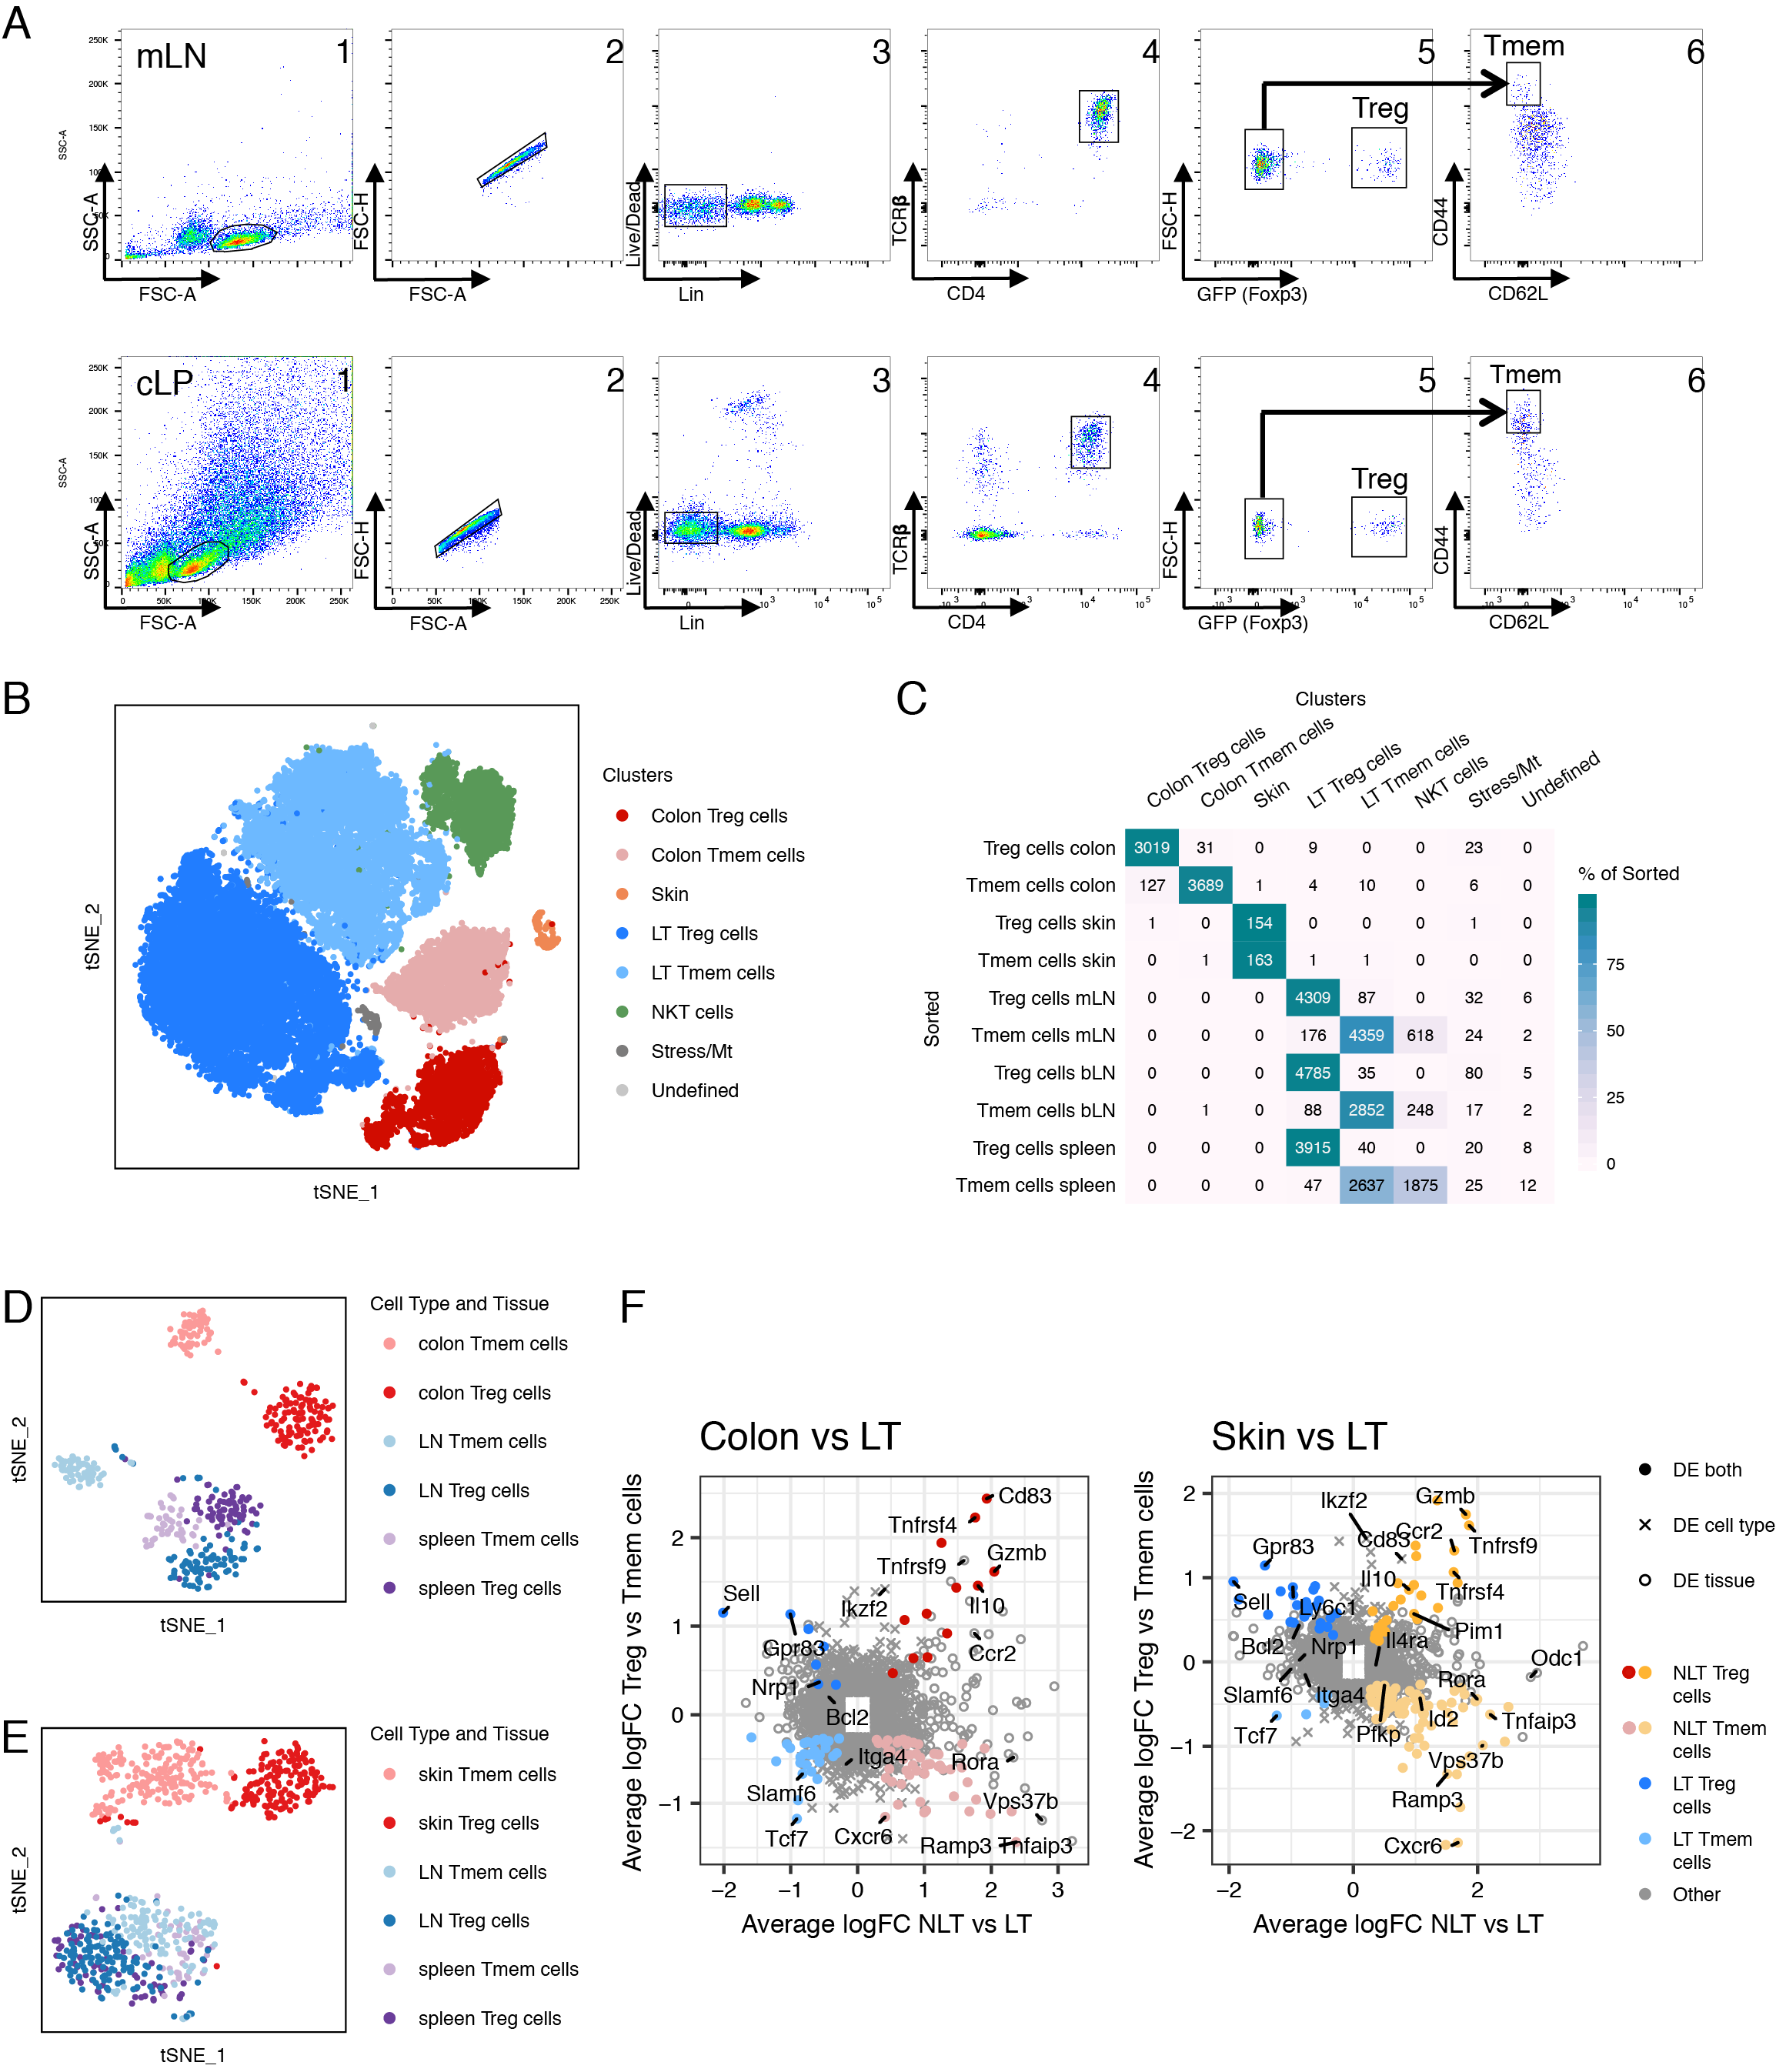
\includegraphics[width=1.0\textwidth]{Appendix1/Figs/appA_fig1.png} % change word in curlies to change figure
\caption[Sorting and identification of Treg and Tmem cells]{\textbf{Sorting and identification of Treg and Tmem cells (Related to Figure~\ref{fig:chap2_fig1}).}\newline\textbf{(A)} Flow cytometry-sorting strategy for sorting Treg and Tmem cells from (top) lymphoid (mLN) and (bottom) non-lymphoid (colonic lamina propria, cLP, as an example) organs. \textbf{(B)} tSNE projection of all 10x dataset cells passing QC, coloured by the resulting graph-based clustering. Cells from the NKT, Stress/Mt and Undefined clusters were removed from further analysis. (Continued on the following page.)}
\label{fig:appA_fig1}
\end{figure}
\begin{figure}[htp!]
  \contcaption{(continued) \textbf{(C)} Number of cells from each cluster in (D) originating from each sorted population. \textbf{(D and E)} Treg and Tmem cells were obtained with the same methodology as in Figure~\ref{fig:chap2_fig1}A, sequenced using Smart-seq2. t-SNE dimensionality reduction represents all sorted cells for each individual batch that passed quality control (see Methods). Colors match cell-type and tissue of origin. \textbf{(F)} Genes defining the identity of Treg and Tmem cells in lymphoid and non-lymphoid tissues, obtained from the Smart-seq2 datasets. Colon and skin were individually compared with their corresponding draining lymph node and spleen cells. Significantly expressed genes in each cell-type-tissue combination have an average log fold-change greater than 0.25 and and adjusted p-value lower than 0.05 (Wilcoxon test).}% Continued caption
\end{figure}

\begin{figure}[ht!]
\centering    
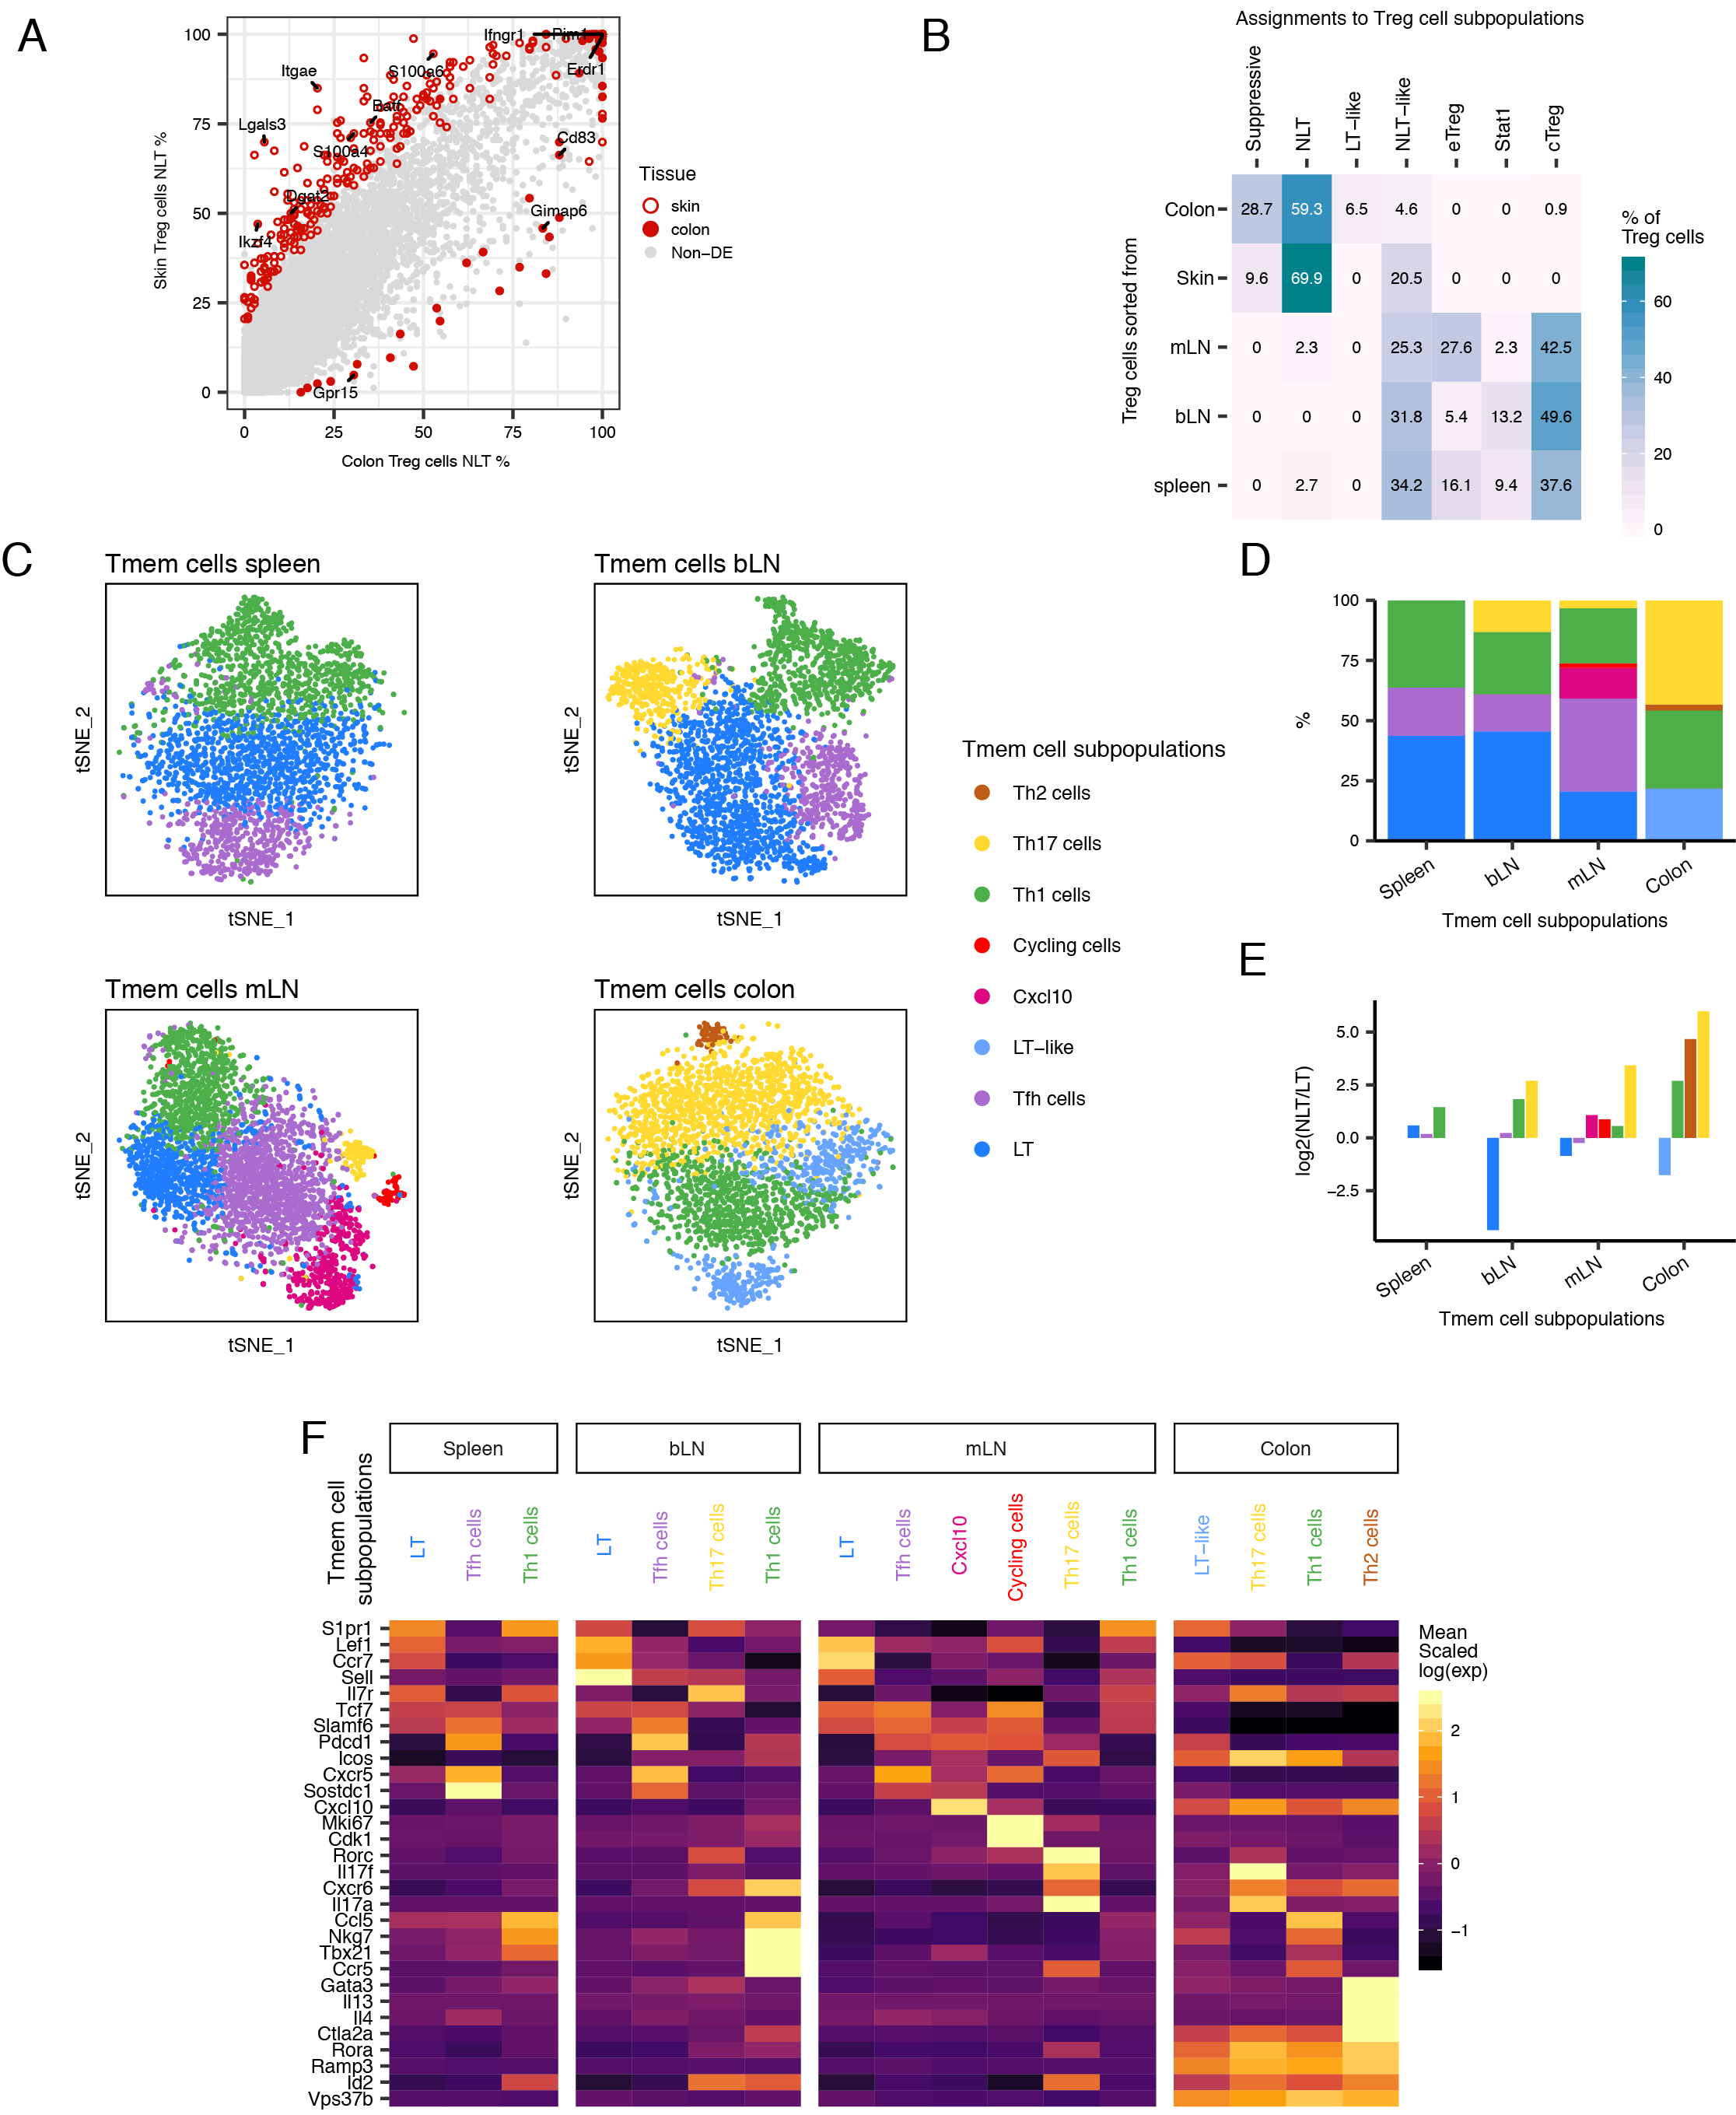
\includegraphics[width=1.0\textwidth]{Appendix1/Figs/appA_fig2.png} % change word in curlies to change figure
\caption[Heterogeneity in SS2 and Tmem cell populations]{\textbf{Heterogeneity in SS2 and Tmem cell populations (Related to Figure~\ref{fig:chap2_fig2}).}\newline\textbf{(A)} Percentage of cells expressing each gene in skin Treg NLT and colon Treg NLT subpopulations in Smart-seq2 data. Genes that are upregulated in the skin Treg NLT subpopulation (log2(FC)>0.25 and adjusted p-value<0.05) are represented by an open circle, and genes upregulated in colon Treg NLT (log2(FC)<(-0.25) and adjusted p-value<0.05) are represented by a filled circle. (Continued on the following page.)}
\label{fig:appA_fig2}
\end{figure}
\begin{figure}[htp!]
  \contcaption{(continued) \textbf{(B)} Matching of Smart-seq2 Treg cells sorted populations to identified Treg subpopulations in the 10x dataset using a logistic regression model (85\% accuracy, see Methods). Table shows the percentage of each sorted population (y-axis) that were labelled as each Treg cluster (x-axis). \textbf{(C)} t-SNE projection of Tmem cells per tissue coloured by subpopulations found using graph-based clustering. \textbf{(D)} Subpopulation marker gene mean expression levels (z-score) per subpopulation. Gene markers exhibit |log2(FC)|>0.25 and adjusted p-value<0.05 in the comparison of each subpopulation versus all the other cells within the same tissue.  Values greater than 2.5 or lower than -1.5 are coloured equally. \textbf{(E)} Relative proportions of Tmem subpopulations within each tissue that revealed heterogeneity. \textbf{(F)} Measure of the NLT/LT signature score in each Tmem subpopulation, measured as the ratio between the number of NLT and LT genes that have been identified as significantly upregulated in each cluster.}% Continued caption
\end{figure}

\begin{figure}[ht!] 
\centering    
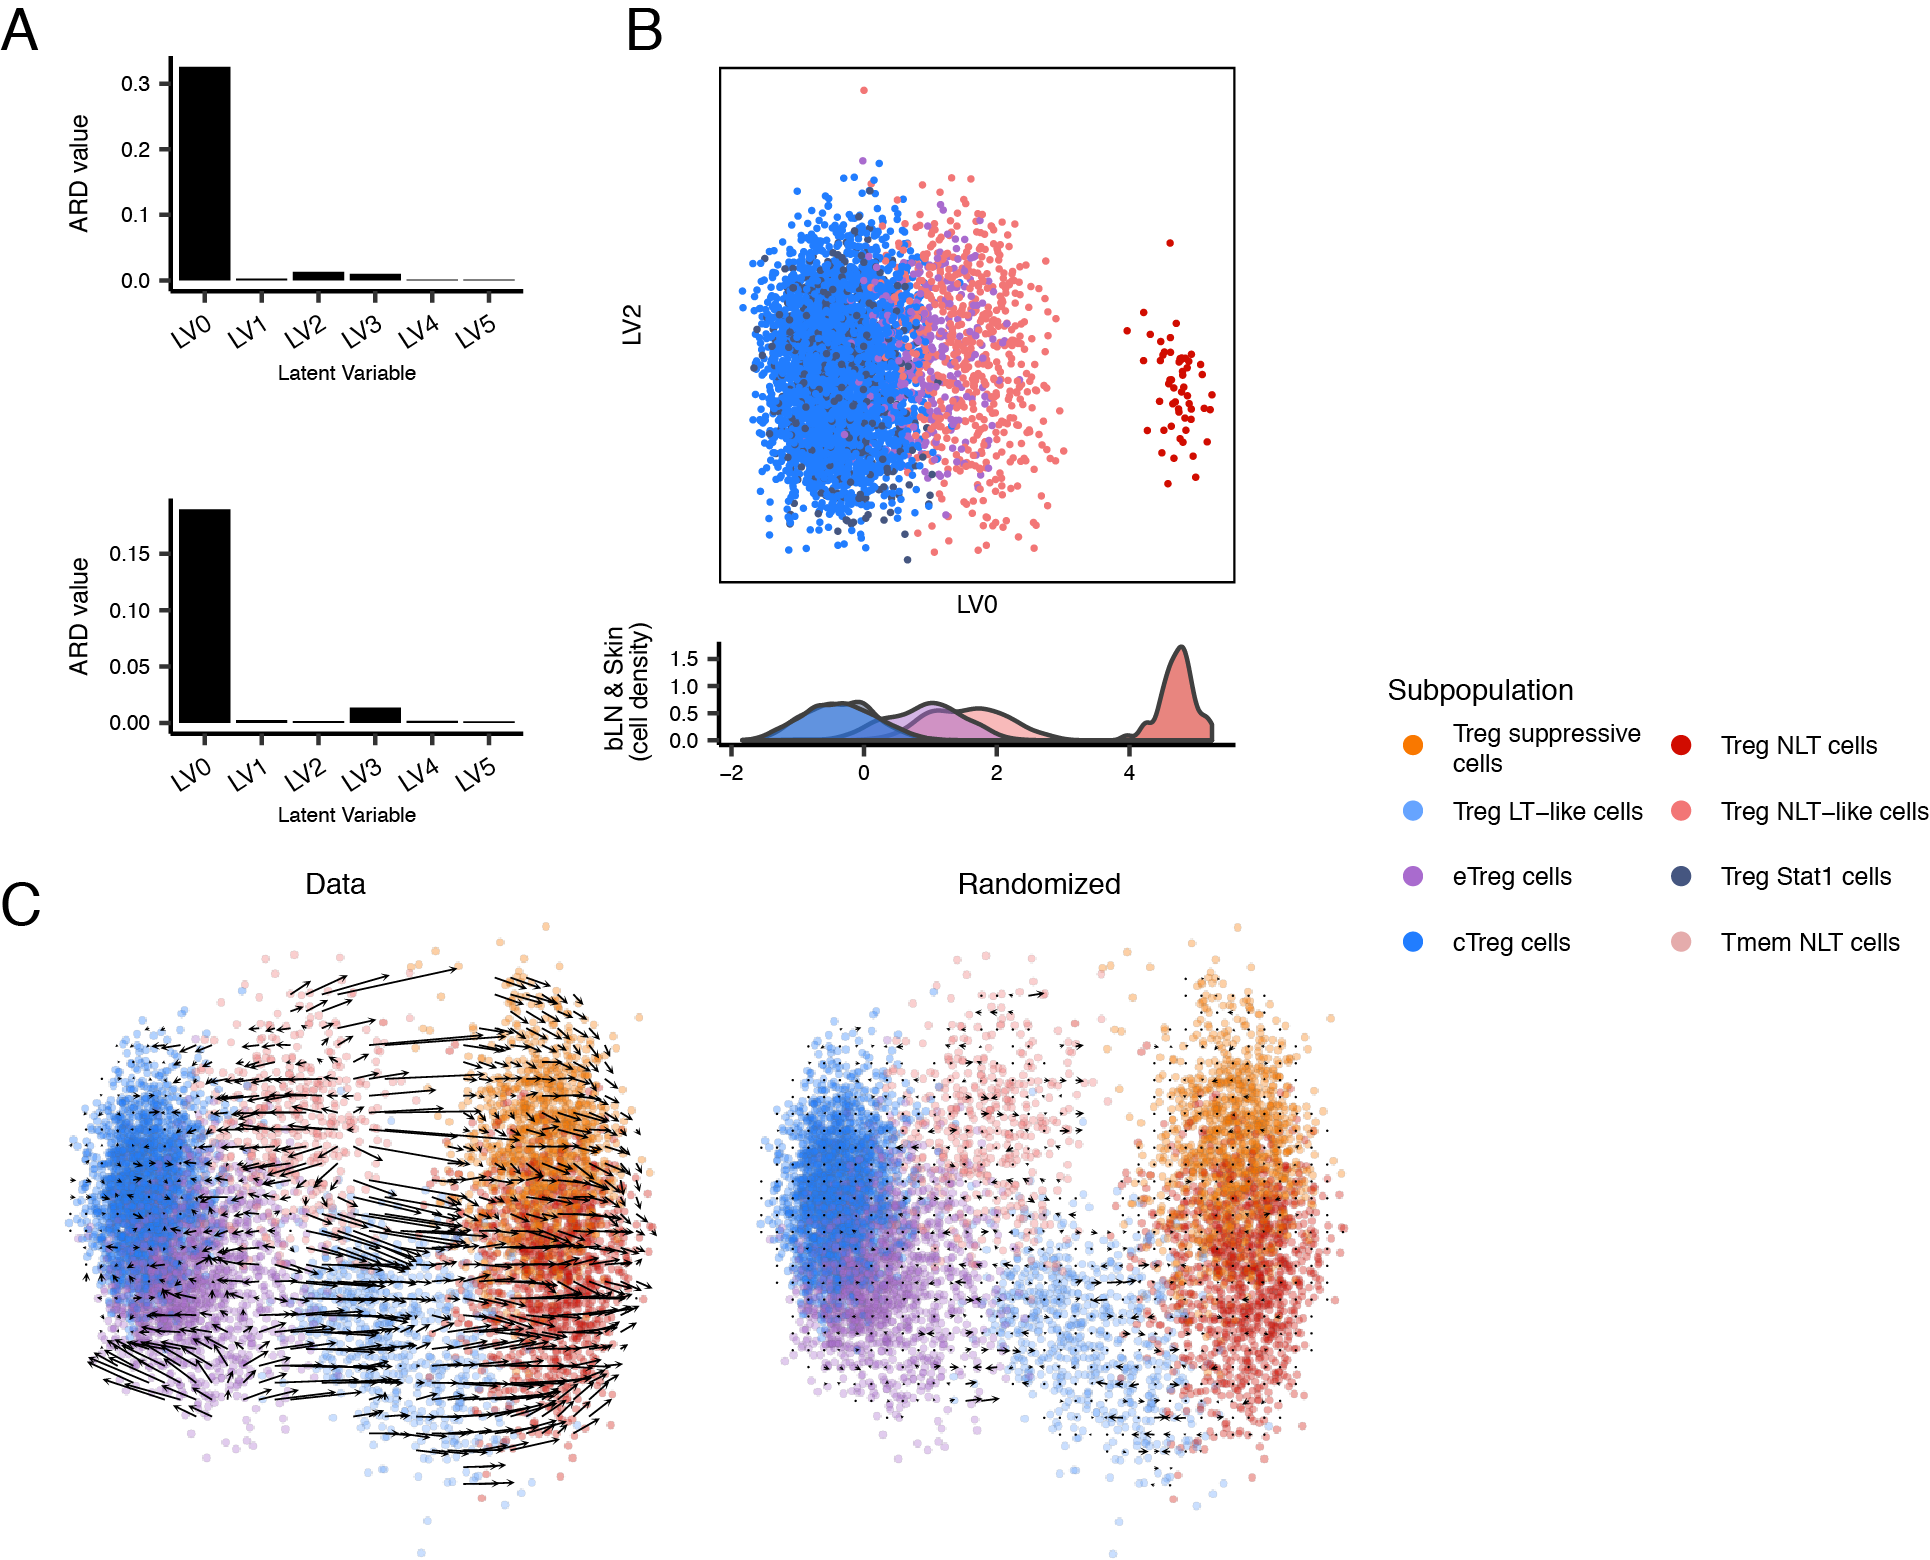
\includegraphics[width=1.0\textwidth]{Appendix1/Figs/appA_fig3.png} % change word in curlies to change figure
\caption[Additional information on BGPLVM for the 10x dataset]{\textbf{Additional information on BGPLVM for the 10x dataset (Related to Figure~\ref{fig:chap2_fig3})}\newline\textbf{(A)} Automatic Relevance Determination (ARD) plots for BGPLVM of Treg in mLN and colon (top, referring to Figure~\ref{fig:chap2_fig3}A), and bLN and skin (bottom, referring to Figure~\ref{fig:appA_fig3}B) datasets. These plots show the relevance of each latent variable extracted from the data. (B) BGPLVM dimensionality reduction of bLN and skin Treg cells from the 10X dataset (top), with a density plot showing the distribution along LV0 of each identified subpopulation (bottom). (C) Velocyto vectorfield overlaid on BGPLVM projection of mLN and colon Treg cells (related to Figure~\ref{fig:chap2_fig3}A).}
\label{fig:appA_fig3}
\end{figure}

\begin{figure}[ht!] 
\centering    
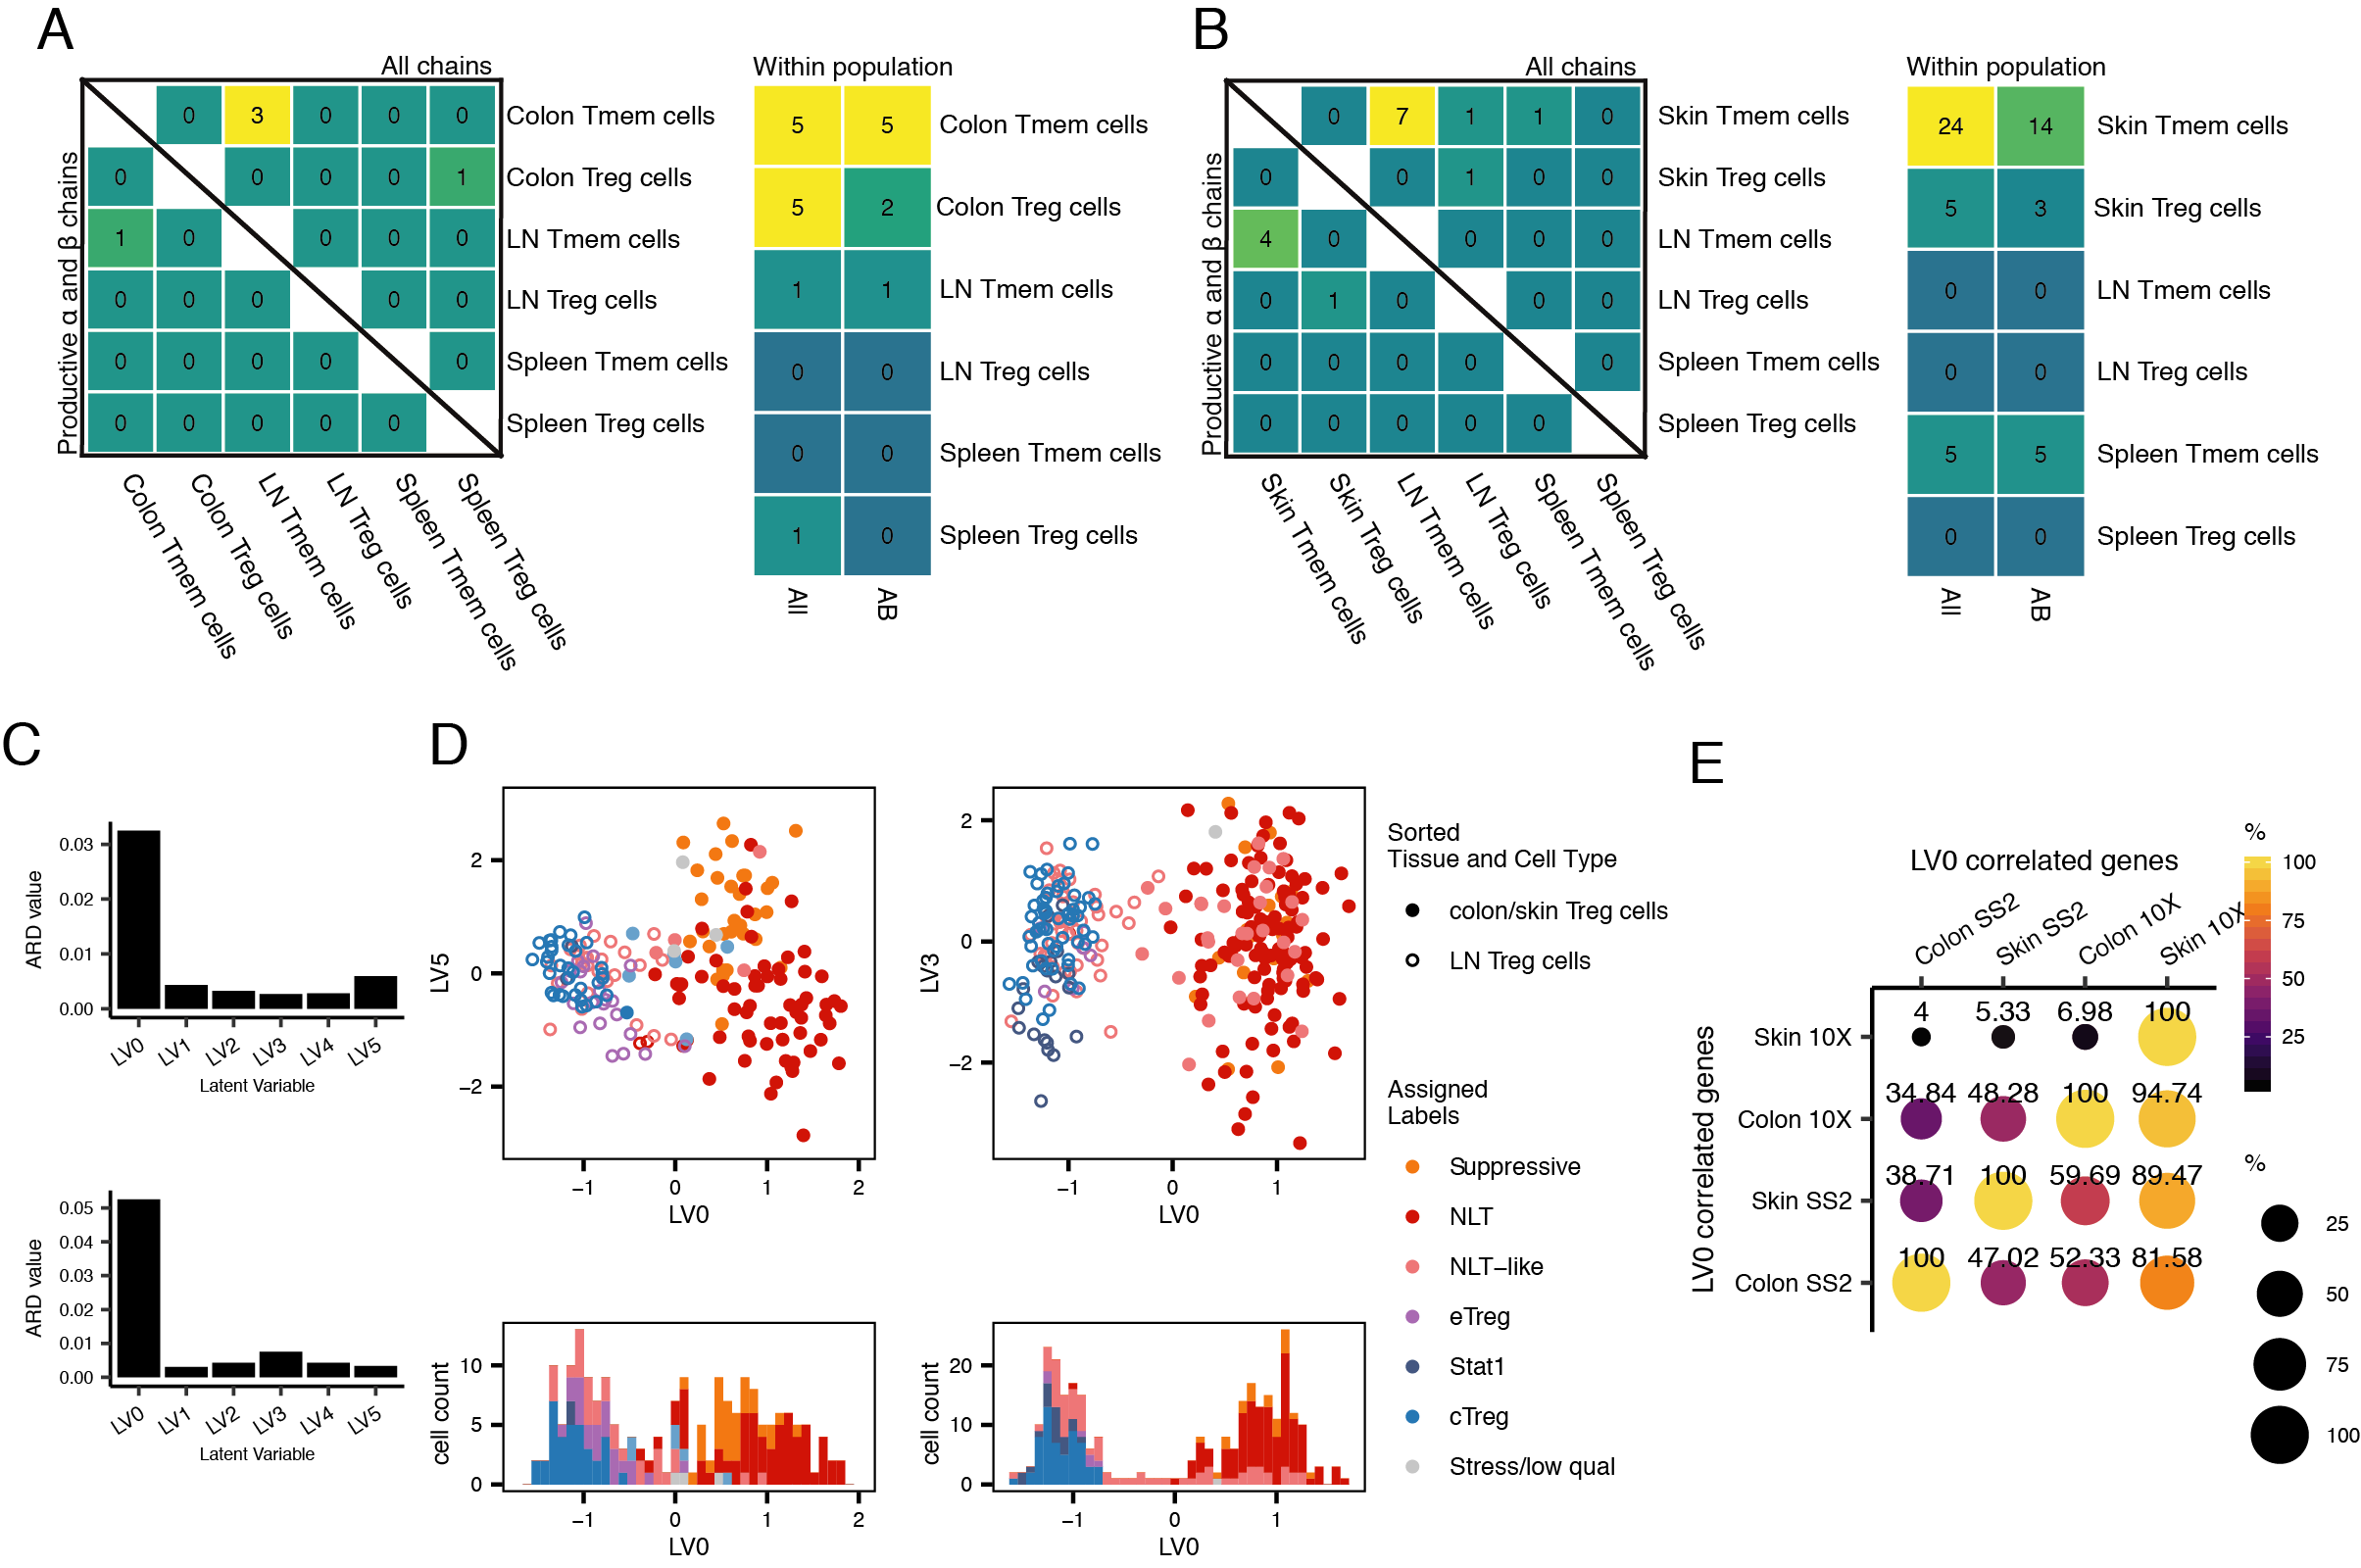
\includegraphics[width=1.0\textwidth]{Appendix1/Figs/appA_fig4.png} % change word in curlies to change figure
\caption[Additional information on BGPLVM for the Smart-seq2 datasets]{\textbf{Additional information on BGPLVM for the Smart-seq2 datasets (Related to Figure~\ref{fig:chap2_fig3})}\newline\textbf{(A and B)} Clonotypes detected using TraCeR in the Smart-seq2 (A) Mouse Colon dataset, or (B) Mouse Skin dataset. In each panel, on the left, number of clonotypes detected spanning different tissues and cell type combinations. Top right half registers all events of TCR chain sharing, bottom left half only considers the sharing of productive ${\upalpha}$ and ${\upbeta}$ TCR chain, and on the right, number of clonotypes detected within each cell type and tissue, considering the sharing of any chain or productive ${\upalpha}$ and ${\upbeta}$. \textbf{(C)} ARD plots for BGPLVM of Smart-seq2 Treg in mLN and colon (top, referring to panel D, left), and bLN and skin (bottom, referring to panel D, right) datasets. \textbf{(D)} BGPLVM dimensionality reduction of Smart-seq2 data of Treg from lymph nodes and non-lymphoid tissues (top), with a histogram plot showing the distribution along LV0 of each subpopulation identified (bottom). mLN and colon Treg are plotted on the left, while bLN and skin Treg are plotted on the right. Cells are coloured by the inferred subpopulation they belong to as per the predictions made in Figure~\ref{fig:appA_fig2}B. \textbf{(E)} Pairwise overlap between the sets of genes with absolute correlation with LV0 greater than 0.25 in each of the four steady-state datasets. The percentages refer to the proportion of the set on the x-axis that is overlapping the set on the y-axis.}
\label{fig:appA_fig4}
\end{figure}

\begin{figure}[pt!] 
\centering    
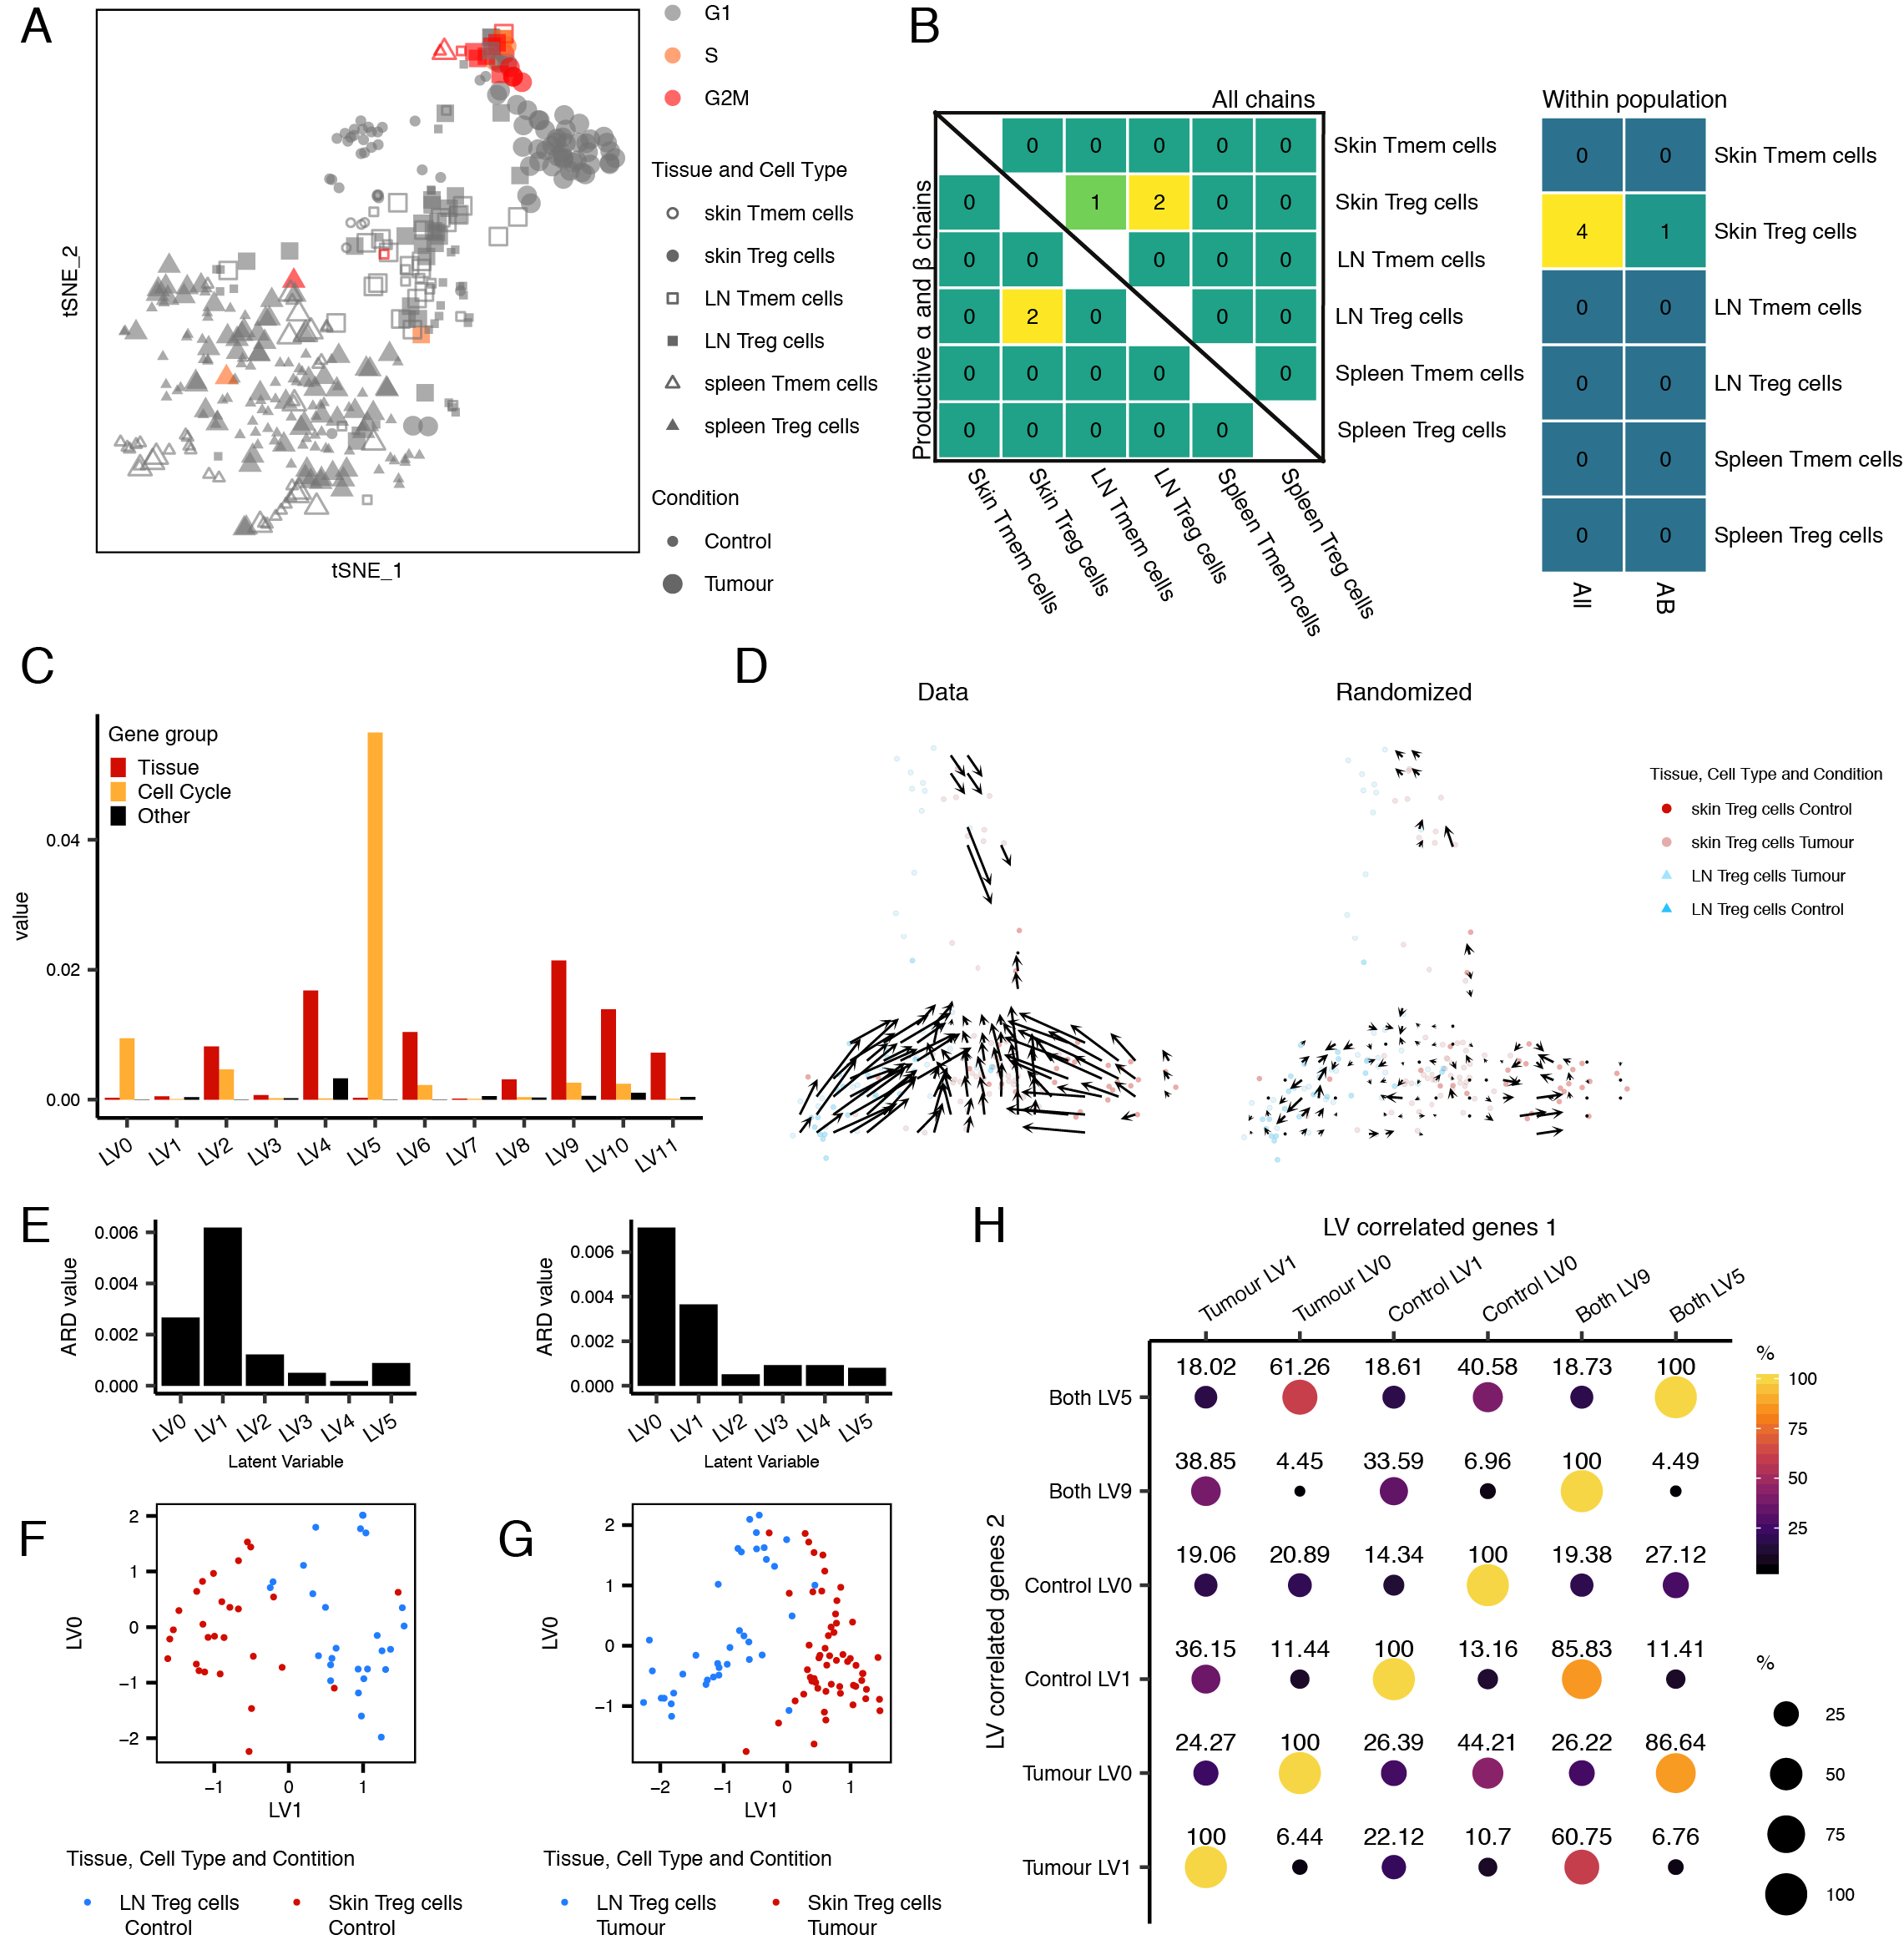
\includegraphics[width=1.0\textwidth]{Appendix1/Figs/appA_fig5.png} % change word in curlies to change figure
\caption[Additional details on the MRD-BGPLVM projection]{\textbf{Additional details on the MRD-BGPLVM projection (Related to Figure~\ref{fig:chap2_fig4}).}\newline\textbf{(A)} t-SNE dimensionality reduction coloured by cell cycle phase in the mouse melanoma dataset. \textbf{(B)} Clonotypes detected using TraCeR in the Mouse Melanoma dataset. On the left, number of clonotypes detected spanning different tissues and cell type combinations. Top right half registers all events of TCR chain sharing, bottom left half only considers the sharing of productive ${\upalpha}$ and ${\upbeta}$ TCR chain. On the right, number of clonotypes detected within each cell type and tissue, considering the sharing of any chain or productive ${\upalpha}$ and ${\upbeta}$. \textbf{(C)} ARD plots for MRD-BGPLVM of Treg in control and melanoma conditions. Colours show effect of gene groups in each obtained latent variable. (Continued on the following page.)}
\label{fig:appA_fig5}
\end{figure}
\begin{figure}[hpt!]
  \contcaption{(continued) \textbf{(D)} Velocyto vectorfield overlaid on MRD-BGPLVM projection of bLN and skin from both Control and Melanoma conditions (related to Figure~\ref{fig:chap2_fig4}D). \textbf{(E)} ARD plots for BGPLVM of Smart-seq2 Treg in bLN and skin in the Control condition (left, related to panel F), and Melanoma condition (bottom, related to panel G). \textbf{(F and G)} BGPLVM projection of bLN and skin in control (F) and melanoma (G) conditions, using the top two latent variables. \textbf{(H)} Pairwise overlap between the sets of genes with absolute correlation with LV0 greater than 0.25 in each subset of the melanoma dataset. The percentages refer to the proportion of the set on the x-axis that is overlapping the set on the y-axis.}% Continued caption
\end{figure}

\begin{figure}[pt!] 
\centering    
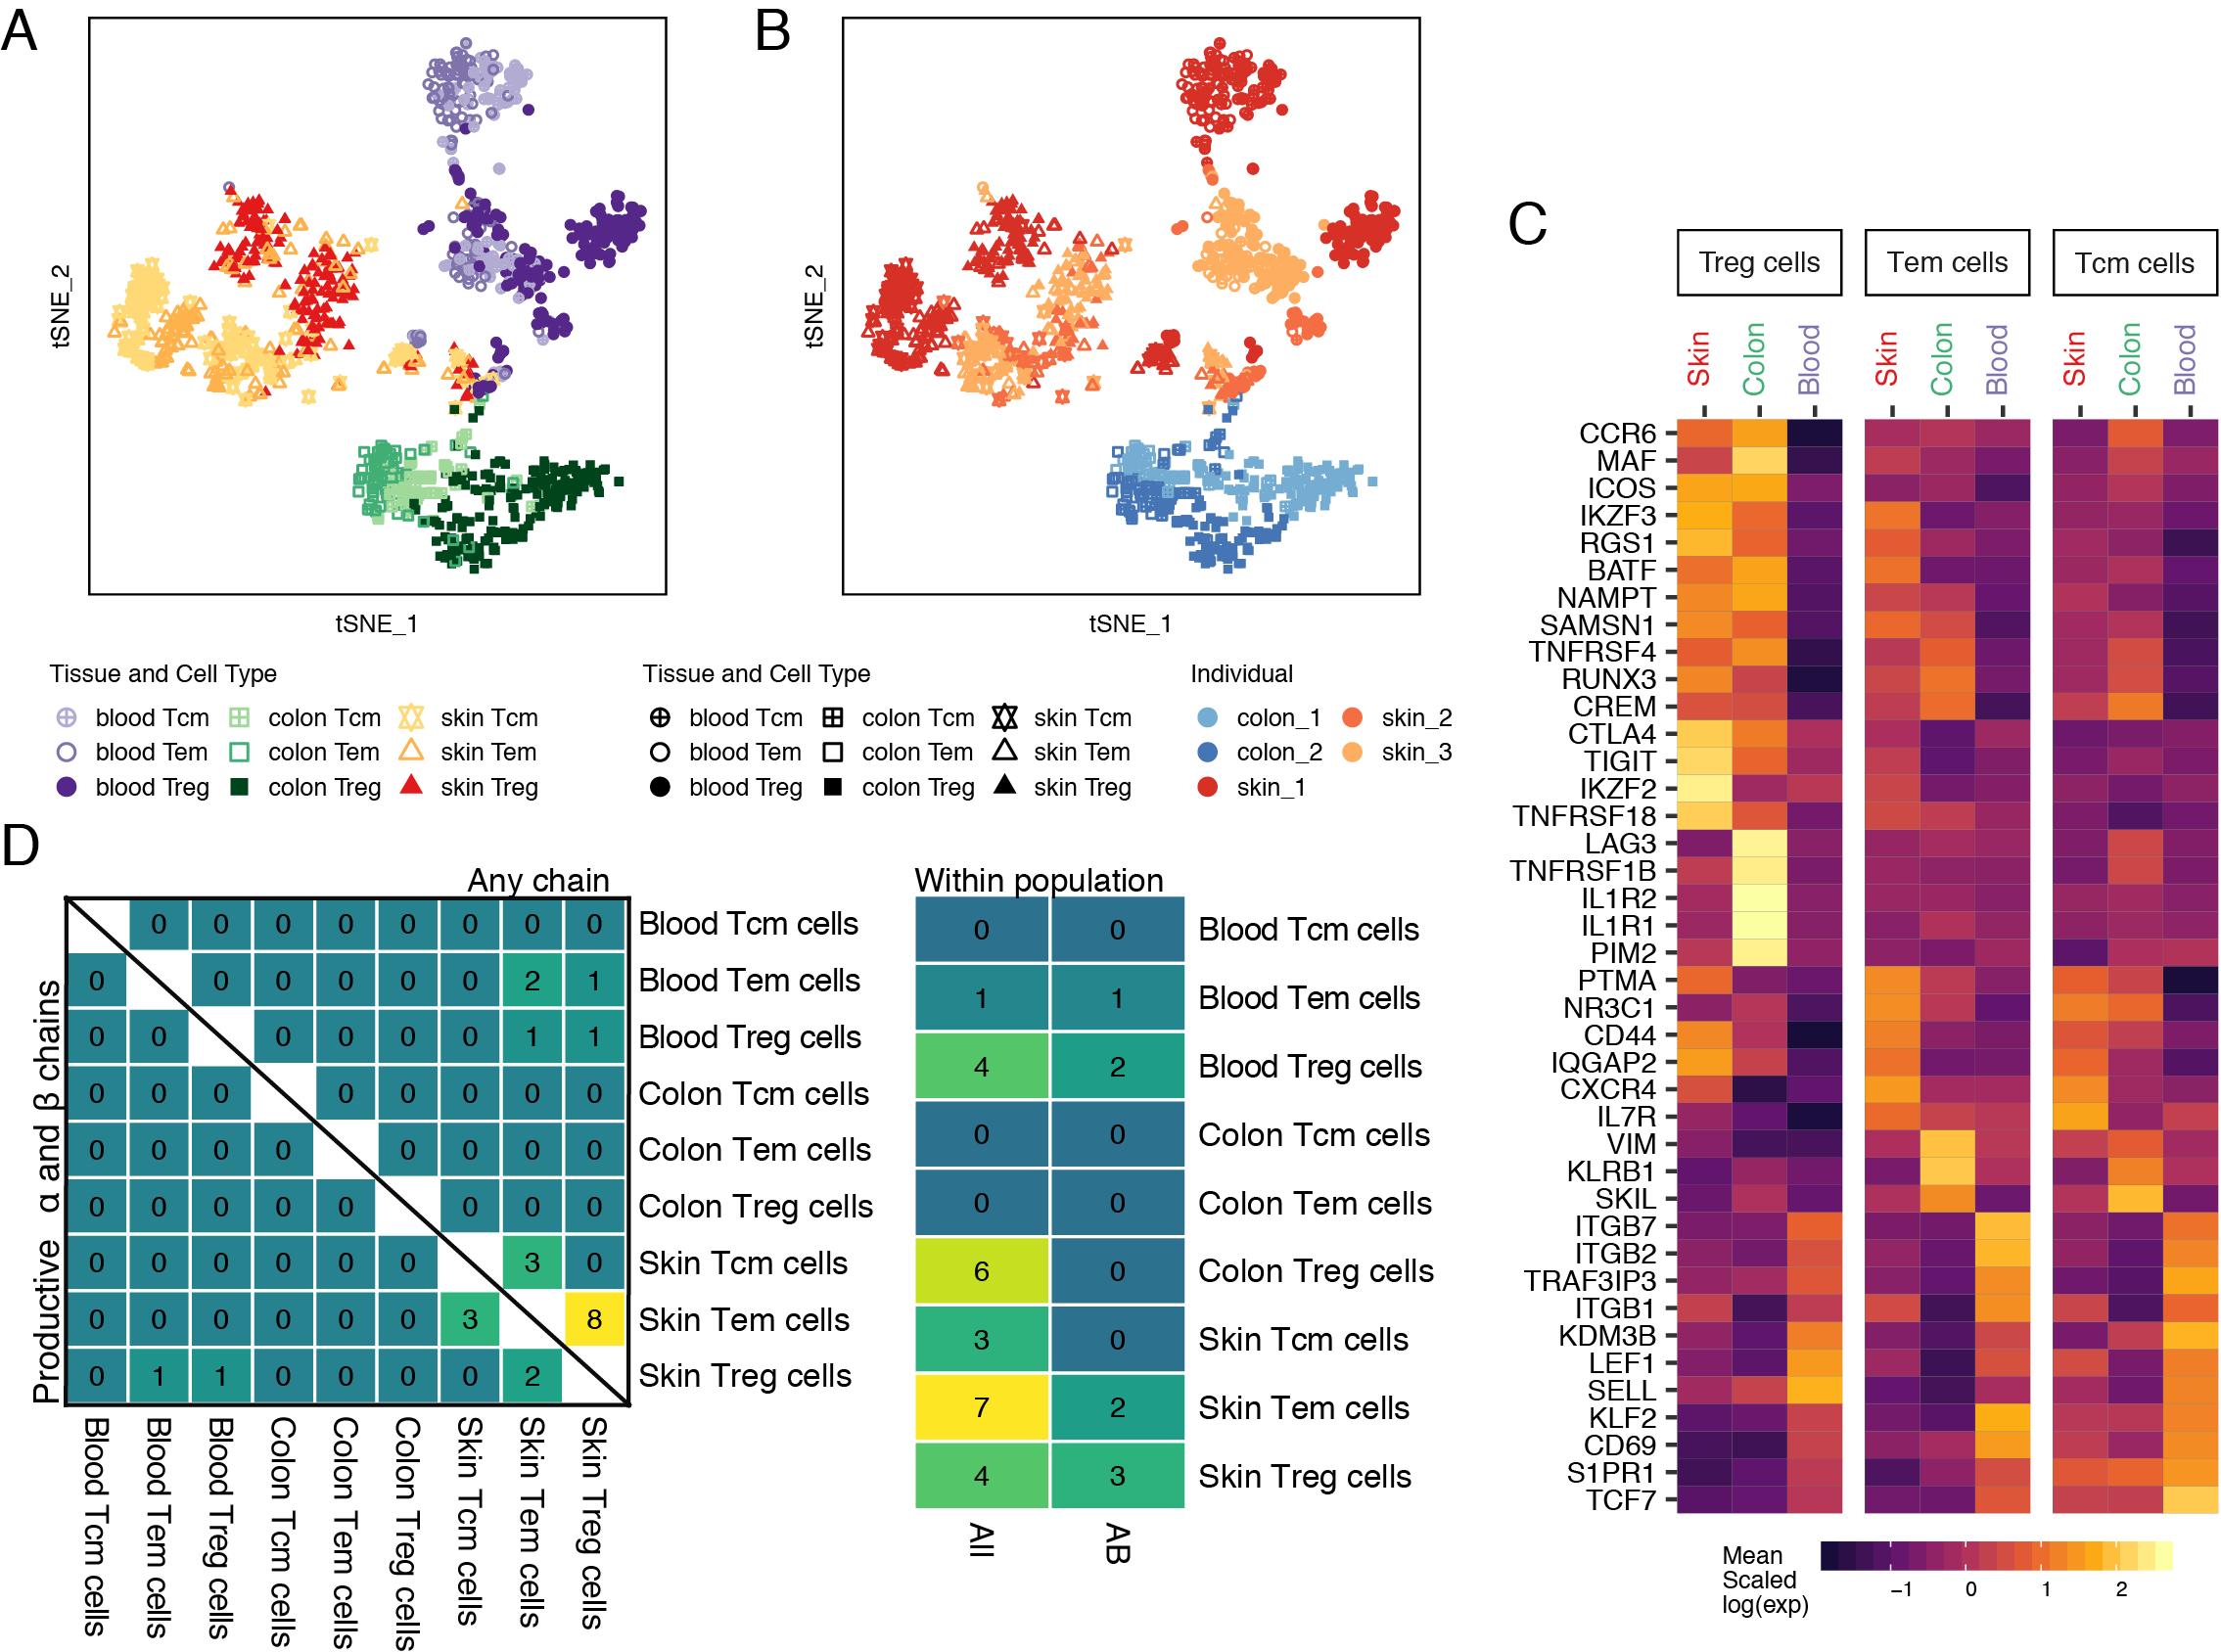
\includegraphics[width=1.0\textwidth]{Appendix1/Figs/appA_fig6.png} % change word in curlies to change figure
\caption[Additional information about the Human Smart-seq2 dataset]{\textbf{Additional information on the Human dataset (Related to Figure~\ref{fig:chap2_fig5}).}\newline\textbf{(A and B)} t-SNE dimensionality reduction. Shapes match cell type and tissue according to legend. Colours match either cell type and tissue (A) or sampled individual (B). \textbf{(C)} Z-score of mean expression levels of identified markers across all sampled cell types and tissues in human. \textbf{(D)} Clonotypes detected using TraCeR in the Human dataset. On the left, number of clonotypes detected spanning different tissues and cell type combinations. Top right half registers all events of TCR chain sharing, bottom left half only considers the sharing of productive ${\upalpha}$ and ${\upbeta}$ TCR chain. On the right, number of clonotypes detected within each cell type and tissue, considering the sharing of any chain or productive ${\upalpha}$ and ${\upbeta}$.}
\label{fig:appA_fig6}
\end{figure}


\pagebreak
\section{Data and Code Accessibility}
\label{sectionA1.3}
scRNA-seq data for this project has been deposited in ArrayExpress under the accession numbers E-MTAB-6072 and E-MTAB-7311. Processed data can be found in \url{https://figshare.com/projects/Treg\_scRNA-seq/38864}, and analysis notebooks can be found in \url{https://github.com/tomasgomes/Treg\_analysis}.


\section{Full author list and contributions}
\label{sectionA1.4}
Ricardo J. Miragaia*, Tomas Gomes*, Agnieszka Chomka, Laura Jardine, Angela Riedel, Ahmed N. Hegazy, Natasha Whibley, Andrea Tucci, Xi Chen, Ida Lindeman, Guy Emerton, Thomas Krausgruber, Jacqueline Shields, Muzlifah Haniffa, Fiona Powrie, Sarah A. Teichmann

*These authors contributed equally to this work

RJM, AC, AH, TK, FP and SAT conceived the project and designed steady-state experiments. RJM and AR designed the melanoma challenge experiments. AC and AH collected cells for steady-state mouse and human colonic datasets. LJ collected cells for human skin dataset. AR induced the melanoma challenge. RJM and AR collected cells for melanoma dataset. RJM performed scRNA-seq. TG, RJM and SAT planned the data analyses. TG and RJM analysed the data. IL performed the TraCeR analysis. RJM, TG, AC, SAT wrote the manuscript. SAT, FP, MH and JS supervised the work and edited manuscripts.

\subsection{Acknowledgements}
We thank V. Proserpio, M. Stubbington, T. Hagai, F.V. Braga, V. Svensson, J. Henriksson for helpful discussions and advice, T. Hagai, R. Vento-Tormo, K. Meyer, J. Park for critical reading of the manuscript, and B. Koppelman for editorial support. We thank WSI Single-cell Genomic Core Facility, WSI Sequencing Facility, WSI Flow Cytometry facilities, K. Polanski, as well as the Kennedy Institute Flow Cytometry Facility, for expert technical advice and assistance. RJM was supported by a PhD Fellowship from the Fundacao para a Ciencia e Tecnologia, Portugal (SFRH/BD/51950/2012), TG by the European Union’s H2020 research and innovation programme “ENLIGHT-TEN” under the Marie Sklodowska-Curie grant agreement 675395. This project was supported by ERC grants ThDEFINE and ThSWITCH. ANH was supported by an EMBO long-term fellowship (ALTF 1161-2012) and a Marie Curie fellowship (PIEF-GA-2012-330621).